\documentclass[10pt,conference]{IEEEtran}
\usepackage{graphicx}
\usepackage{amsmath}
\usepackage{amssymb}
\usepackage{booktabs}
\usepackage{array}
\usepackage{multirow}
\usepackage{tikz}
\usetikzlibrary{arrows.meta,positioning,fit,shapes.geometric}
\usepackage{hyperref}
\usepackage{xcolor}
\usepackage{caption}
\usepackage{subcaption}
\usepackage{listings}
\usepackage{balance}

\graphicspath{
  {../assets/figma/}
  {../../runs/runs/yolo_ui_detector/runs/yolo_ui_detector/}
  {../../runs/crop_violation_classifier/crop_classifier/}
}

\hypersetup{
    colorlinks=true,
    linkcolor=blue,
    urlcolor=blue,
    citecolor=blue
}

\lstdefinestyle{jsonstyle}{
    basicstyle=\ttfamily\scriptsize,
    breaklines=true,
    columns=fullflexible,
    frame=single,
    numbers=none,
    backgroundcolor=\color{gray!5}
}

\renewcommand{\arraystretch}{1.15}

\begin{document}

\title{Agentic Accessibility Auditor (Axion): An AI-Driven Pipeline for\\ Automated Android Mobile UI Accessibility Auditing}

\author{
\IEEEauthorblockN{Muhammad Noor ul Haq}
\IEEEauthorblockA{
\textit{NCRA-UAV Dependability Lab} \\
\textit{FAST NUCES, Islamabad} \\
Islamabad, Pakistan \\
i232520@isb.nu.edu.pk
}
\and
\IEEEauthorblockN{Salar Khan}
\IEEEauthorblockA{
\textit{NCRA-UAV Dependability Lab} \\
\textit{FAST NUCES, Islamabad} \\
Islamabad, Pakistan \\
i232607@isb.nu.edu.pk
}
\and
\IEEEauthorblockN{Ayesha Naveed}
\IEEEauthorblockA{
\textit{NCRA-UAV Dependability Lab} \\
\textit{FAST NUCES, Islamabad} \\
Islamabad, Pakistan \\
i233068@isb.nu.edu.pk
}
}

\maketitle

\begin{abstract}
Accessibility evaluation of Android mobile applications remains largely manual, slow, and inconsistent, and existing automated tools detect only a fraction of the structural issues that affect users with visual, motor, auditory, or cognitive impairments. This paper presents the \emph{Agentic Accessibility Auditor}, branded \textbf{Axion}, a working prototype developed over an eight-week summer internship at FAST--NUCES that combines an Android UI screenshot with its UIAutomator XML hierarchy to automatically detect accessibility violations, map them to WCAG~2.2~AA-aligned guidelines, and generate developer-facing explanations and fixes using a large language model (LLM) agent. The system is implemented as a six-layer pipeline -- input, parsing, rule checking, agentic explanation, report generation, and evaluation -- exposed through a FastAPI backend and a React/Tailwind web dashboard with authentication and per-user audit history. A deterministic rule engine implements 30 detection rules (R01--R30) mapped to 30 accessibility guidelines (G01--G30). Two supplementary computer-vision modules were trained and integrated: a YOLO11-based screenshot-only UI-element detector that provides a fallback when no XML hierarchy is available, and a Swin-Tiny-backboned multi-label crop classifier that confirms six pixel-dependent rules from rendered screenshots. The system was developed and tuned on the 7{,}068-screen MASC dataset and evaluated, without further tuning, on a disjoint 1{,}698-screen Rico holdout set, on which the rule engine reports a mean of 31.7 violations per screen and a mean accessibility score of 32.0/100, and the YOLO detector achieves mAP50 of 0.2546 (up from a zero-shot baseline of 0.0258), while the crop classifier reaches a Rico holdout macro-F1 of 0.22, the best result across a 33-backbone comparison sweep. We describe the full system design, dataset strategy, evaluation methodology, and empirical results, and close with a discussion of limitations and directions for future work.
\end{abstract}

\begin{IEEEkeywords}
accessibility testing, Android, WCAG, agentic AI, large language models, UI automation, YOLO, vision transformers, software engineering, human--computer interaction
\end{IEEEkeywords}

\section{Introduction}

Mobile applications are expected to be usable by people with a wide range of abilities, yet accessibility evaluation in industry practice is still predominantly manual, ad hoc, and dependent on the reviewer's familiarity with the Web Content Accessibility Guidelines (WCAG). Screen-reader walkthroughs and manual checklists do not scale to the pace of continuous mobile development, and purely visual (screenshot-only) automated tools cannot reliably detect structural issues such as missing content descriptions, duplicate accessible labels, undersized touch targets, or unlabeled input fields, because these properties are encoded in the underlying UI hierarchy rather than in pixels alone. Existing automated scanners typically apply a small, fixed rule set and stop at a raw diagnostic code, leaving a developer with no explanation of \emph{why} an issue matters to a real user or \emph{how} to fix it in their own layout XML.

This project set out to close that gap by treating Android accessibility auditing as a two-input task: a rendered \textbf{screenshot} and its corresponding \textbf{UIAutomator XML} view hierarchy -- the same structured tree that Android's own TalkBack screen reader consumes. By parsing the XML into a structured component representation and applying a deterministic rule engine, the system detects concrete, reproducible violations. An \emph{agentic} large language model (LLM) layer then explains each rule-detected violation in plain English, describes its impact on users with disabilities, and proposes a concrete developer fix -- but is explicitly and architecturally constrained never to invent violations that the rule engine did not detect. The end result is packaged into an HTML/PDF audit report and surfaced through a branded web dashboard, \textbf{Axion}, complete with user accounts and a persistent history of past audits.

The project was carried out by a three-person intern team over an eight-week internship, with each member owning a primary pipeline layer while collaborating on shared artifacts: the rule engine, the JSON schema contracts that let the three layers integrate independently, and the requirements/design documentation. What began as a Must-Have/Should-Have/Stretch-tiered plan concluded with every tier delivered, including two originally-optional computer-vision models that were fully trained, evaluated on unseen data, and wired into the production backend in the project's final week. This report documents the objectives, system architecture, implementation, dataset and evaluation strategy, and the empirical results obtained on both the development dataset and an unseen holdout set, followed by a discussion of limitations and future work.

\section{Background}

\textbf{WCAG 2.2 AA.} The project's 30 accessibility guidelines (G01--G30) are each aligned to a specific WCAG 2.2 success criterion -- for example G01 (missing accessible label) to 4.1.2 Name/Role/Value, G04 (small touch target) to 2.5.5 Target Size, and G09 (low contrast) to 1.4.3 Contrast (Minimum) -- so every finding in the tool carries a traceable standards reference rather than an ad hoc justification.

\textbf{UIAutomator and the Android accessibility tree.} Android exposes a structured view hierarchy via \texttt{UIAutomator}, in which every node carries properties such as \texttt{class}, \texttt{text}, \texttt{content-desc}, \texttt{clickable}, \texttt{enabled}, \texttt{focusable}, \texttt{resource-id}, and pixel \texttt{bounds}. This tree is exactly what a screen reader relies on to announce and navigate a screen, which makes it the most direct available signal for structural accessibility problems -- but it is unavailable for apps that intentionally suppress or obfuscate their accessibility tree, motivating the project's screenshot-only fallback module.

\textbf{Agentic LLM layers.} A growing body of recent work applies LLMs directly as the accessibility-error \emph{detector} on mobile UIs -- ScreenAudit~\cite{screenaudit} prompts an LLM over screen-reader traversal output to find accessibility errors, and Insight~\cite{insight} uses an LLM to interpret and narrate live screens for blind and low-vision users. This project takes a deliberately different position: a language model is most reliable as an \emph{explainer} layered over a deterministic source of truth rather than as the detector itself. This separation was adopted as a hard design constraint from the outset: the rule engine is the sole detector of violations, deterministic and reproducible by construction, while the LLM agent is restricted to explaining, contextualizing, and recommending fixes for issues it is handed, with an explicit anti-hallucination check verifying that every explanation returned by the model corresponds to a real violation ID that was actually sent to it.

\section{Problem Statement and Objectives}

Android accessibility evaluation is manual, slow, and inconsistent, and existing automated tools miss structural issues that only the UI hierarchy exposes. There is a need for an automated, explainable, developer-friendly system that combines a screenshot, the UI hierarchy, deterministic rule checks, and AI-generated recommendations into a single audit workflow. The concrete objectives set for the internship were to:

\begin{itemize}
    \item Accept a paired Android UI screenshot and UIAutomator XML file through a web interface;
    \item Parse the XML into structured component records (\texttt{class}, \texttt{bounds}, \texttt{text}, \texttt{content-desc}, \texttt{clickable}, \texttt{enabled}, \texttt{focusable}, \texttt{resource-id});
    \item Implement deterministic rule-based accessibility checks for common Android UI issues;
    \item Map every detected issue to an accessibility guideline category with a WCAG reference and severity;
    \item Use an agentic explanation layer to produce plain-English explanations and developer-facing fixes, without inventing new issues;
    \item Generate an HTML/PDF audit report with an issue summary, affected elements, severity, and recommendations;
    \item Evaluate the tool on at least 25--40 Android screens and document the results.
\end{itemize}

Priorities were tiered into a Minimum Viable Product (parser $\rightarrow$ R01--R10 $\rightarrow$ LLM explanations $\rightarrow$ HTML/PDF report $\rightarrow$ Axion Upload/Dashboard/Report $\rightarrow$ authentication and per-user records $\rightarrow$ Docker deployment $\rightarrow$ evaluation on 25--40 screens), a Should-Have tier (R11--R20, dashboard filtering, batch processing), and a Stretch tier (R21--R30, a multi-label pixel-level crop classifier, a screenshot-only YOLO fallback detector, and interactive report highlighting). By project close, all three tiers -- including both stretch computer-vision models -- were implemented and wired into the production pipeline, and 99 of 99 tracked functional and non-functional requirements were marked Done in the project's requirements traceability matrix.

\section{System Architecture}

The system is structured as a six-layer pipeline in which every stage produces a versioned, schema-validated JSON artifact consumed by the next stage. This artifact-oriented design let the three interns develop and test their modules independently against agreed contracts rather than a shared in-memory state, and made regression testing tractable at dataset scale.

\begin{figure}[!t]
\centering
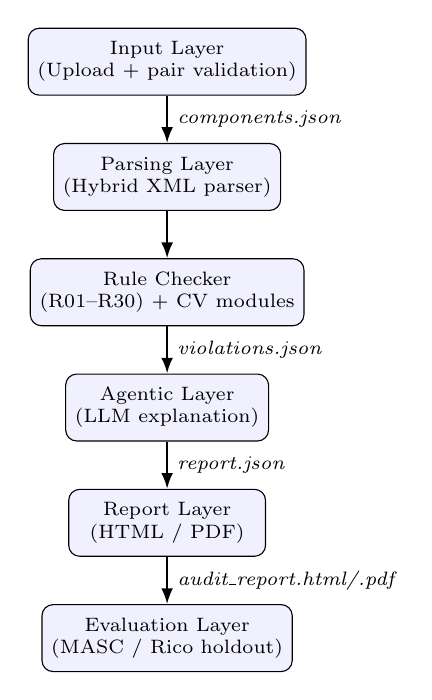
\begin{tikzpicture}[
    node distance=6mm and 6mm,
    box/.style={draw, rounded corners, minimum width=2.5cm, minimum height=0.85cm, align=center, fill=blue!6, font=\scriptsize},
    art/.style={font=\scriptsize\itshape, align=center},
    arrow/.style={-{Latex[length=2mm]}, thick}
]
\node[box] (input) {Input Layer\\(Upload + pair validation)};
\node[box, below=of input] (parse) {Parsing Layer\\(Hybrid XML parser)};
\node[box, below=of parse] (rules) {Rule Checker\\(R01--R30) + CV modules};
\node[box, below=of rules] (agent) {Agentic Layer\\(LLM explanation)};
\node[box, below=of agent] (report) {Report Layer\\(HTML / PDF)};
\node[box, below=of report] (eval) {Evaluation Layer\\(MASC / Rico holdout)};

\draw[arrow] (input) -- (parse) node[midway, right, art] {components.json};
\draw[arrow] (parse) -- (rules) node[midway, right, art] {};
\draw[arrow] (rules) -- (agent) node[midway, right, art] {violations.json};
\draw[arrow] (agent) -- (report) node[midway, right, art] {report.json};
\draw[arrow] (report) -- (eval) node[midway, right, art] {audit\_report.html/.pdf};
\end{tikzpicture}
\caption{Six-layer pipeline architecture. Each layer emits a schema-validated JSON artifact consumed by the next stage.}
\label{fig:pipeline}
\end{figure}

Figure~\ref{fig:pipeline} shows the logical data flow: a screenshot and UIAutomator XML pair enters the Input Layer; the Parsing Layer converts the XML into \texttt{components.json}; the Rule Checker (optionally confirmed by the crop classifier, or entirely substituted by the YOLO detector when XML is unavailable) produces \texttt{violations.json}; the Agentic Layer enriches each violation into \texttt{report.json}; the Report Layer renders \texttt{audit\_report.html}/\texttt{.pdf}; and the Evaluation Layer aggregates results across the MASC and Rico holdout datasets.

At the physical level, the system is a FastAPI backend (\texttt{backend/}) exposing three route groups -- \texttt{/api/v1/audit/*} for the pipeline, \texttt{/auth/*} for authentication, and \texttt{/records/*} for per-user history -- behind a React 19 + Vite + Tailwind CSS frontend (\texttt{frontend/}), all orchestrated with Docker Compose (\texttt{backend}, \texttt{auditor}, and \texttt{frontend} services on an internal bridge network, \texttt{auditor-network}). Table~\ref{tab:stack} summarizes the technology stack.

\begin{table}[!t]
\caption{Technology stack summary.}
\label{tab:stack}
\centering
\scriptsize
\begin{tabular}{@{}p{1.9cm}p{5.7cm}@{}}
\toprule
\textbf{Layer} & \textbf{Technology} \\
\midrule
Backend API & Python 3.11, FastAPI 0.110+ \\
XML parsing & \texttt{lxml} / \texttt{xml.etree.ElementTree} \\
Image handling & PIL, OpenCV \\
Rule engine & Pure Python, no ML dependency \\
Object detection & Ultralytics YOLO11s (screenshot-only fallback) \\
Crop classification & \texttt{timm} \texttt{swin\_tiny\_patch4\_window7\_224}, PyTorch \\
Agent / LLM & Groq (\texttt{llama-3.3-70b-versatile}), with Anthropic/OpenAI/Gemini as alternates \\
Report rendering & Jinja2 (HTML) + Playwright/Chromium (PDF) \\
Frontend & React 19, Vite, Tailwind CSS, React Router \\
Auth & JWT (HS256), bcrypt, SMTP OTP, Google OAuth \\
Deployment & Docker, Docker Compose (bridge network) \\
Testing & pytest, FastAPI \texttt{TestClient} \\
\bottomrule
\end{tabular}
\end{table}

\section{Dataset Strategy}

Two datasets anchor the project's development-versus-generalization strategy, summarized in Table~\ref{tab:datasets}. \textbf{MASC} (Mobile App Screens Classification dataset)~\cite{masc-kaggle} supplies 7{,}068 paired screenshot/XML screens across ten UI categories (chat, home, list, login, maps, menu, profile, search, settings, welcome), split 70\%/15\%/15\% into train/val/test (4{,}943/1{,}056/1{,}069 screens respectively) and used for parser development, rule tuning, and all model training. \textbf{Rico holdout}~\cite{rico,rico-kaggle} is a 1{,}698-screen subset of the Rico UI corpus, kept strictly disjoint from MASC and reserved for final, unseen evaluation; it was never used to tune rules or train either computer-vision model, enforced structurally where possible -- for instance, the YOLO dataset configuration for Rico points its \texttt{train}, \texttt{val}, and \texttt{test} splits all at the same held-out image set, so the model cannot accidentally be trained on it.

\begin{table}[!t]
\caption{Dataset strategy: MASC (development) vs. Rico holdout (unseen evaluation).}
\label{tab:datasets}
\centering
\scriptsize
\begin{tabular}{@{}p{1.3cm}p{1.0cm}p{2.2cm}p{2.1cm}@{}}
\toprule
\textbf{Dataset} & \textbf{Size} & \textbf{Split} & \textbf{Purpose} \\
\midrule
MASC & 7{,}068 pairs & 4{,}943 / 1{,}056 / 1{,}069 (train/val/test) & Development, parser tuning, rule development, model training \\
Rico holdout & 1{,}698 pairs & 100\% held out & Final unseen evaluation -- no tuning \\
\bottomrule
\end{tabular}
\end{table}

Supplementary real-device collection was also supported through the standard Android tool chain (\texttt{adb exec-out screencap}, \texttt{adb shell uiautomator dump}, \texttt{adb shell wm size/density}), for cases where a new, uncatalogued app needed to be audited directly from an emulator or physical device.

\section{Implementation}

\subsection{Input Layer and Pair Validation}
Axion's Upload screen (Fig.~\ref{fig:upload}) accepts a screenshot (PNG/JPG) and, optionally, a matching UIAutomator XML file through a sequential drop zone. A four-check Validation Status panel (screenshot detected, XML detected, valid pair, ready for analysis) gates the ``Start Audit'' action, and the backend independently re-validates that the two filenames share a stem or numeric screen ID before the pipeline runs, rejecting mismatched pairs with a clear error. The XML upload is optional: if it is missing, malformed, or parses to zero components, the pipeline transparently falls back to the screenshot-only YOLO detector described in Section~\ref{sec:yolo}.

\begin{figure}[!t]
\centering
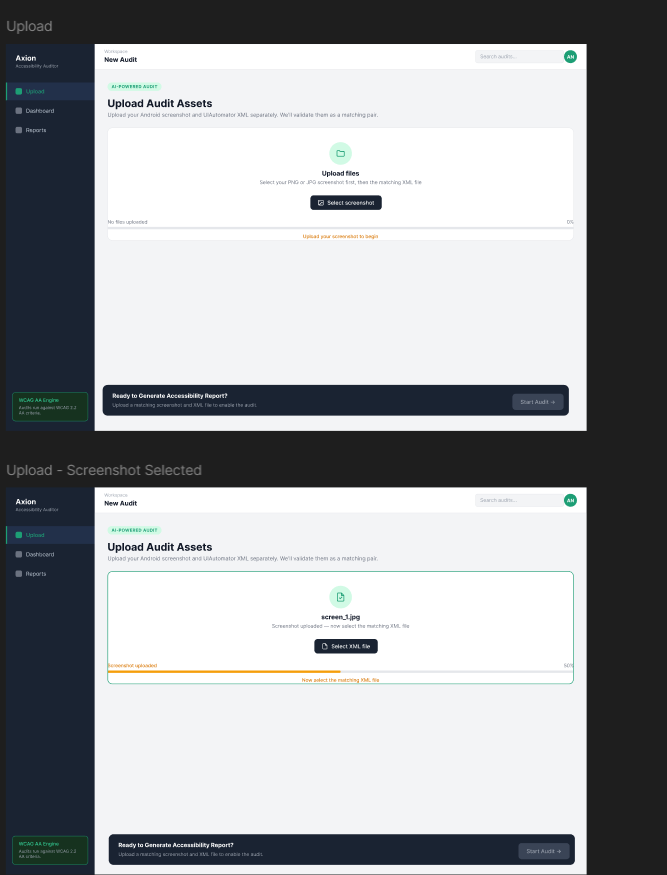
\includegraphics[width=\linewidth]{figma-04-upload-progress-states.png}
\caption{Axion Upload screen: sequential screenshot/XML drop zone with live validation progress.}
\label{fig:upload}
\end{figure}

\begin{figure}[!t]
\centering
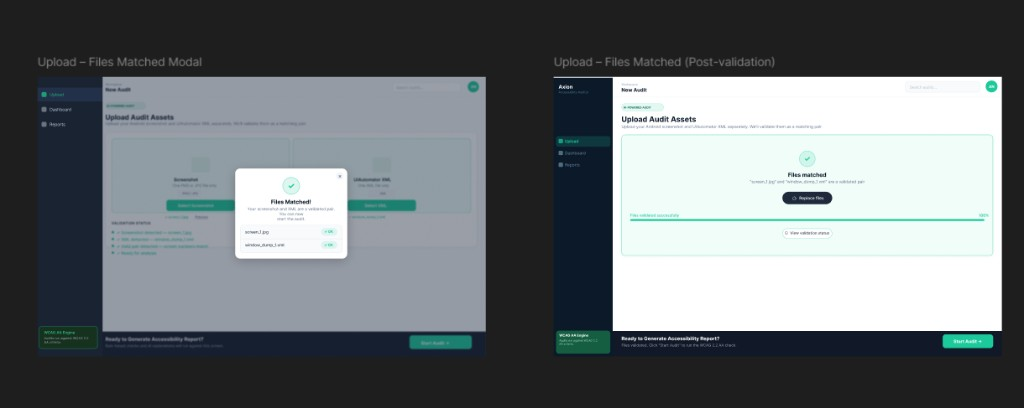
\includegraphics[width=\linewidth]{figma-08-upload-files-matched.png}
\caption{Files Matched confirmation modal shown once a screenshot/XML pair validates, with the Validation Status checklist visible beneath.}
\label{fig:filesmatched}
\end{figure}

\subsection{Parsing Layer: Hybrid XML Parser}
\texttt{src/parser.py} implements a hybrid, single-traversal parser that recognizes four XML dialects encountered across the project's datasets: native \texttt{UIAutomator} bounds syntax (\texttt{[l,t][r,b]}), \texttt{MASC}'s wrapper-nested widgets with numeric bounds, \texttt{Rico}'s space-separated bounds, and generic uploads. For every node it extracts the required fields (\texttt{class}, \texttt{text}, \texttt{content-desc}, \texttt{resource-id}, \texttt{clickable}, \texttt{enabled}, \texttt{focusable}, \texttt{bounds}) plus an extended set of fields discovered necessary during rule development -- \texttt{focus\_order} and \texttt{parent\_id} (depth-first traversal order, used for focus-order and hierarchy rules), \texttt{long\_clickable}/\texttt{scrollable} (gesture heuristics), \texttt{media\_type}, \texttt{is\_dialog}, and \texttt{hint}/\texttt{input\_type}/\texttt{password}/\texttt{label\_for} (input labelling). Malformed or incomplete XML is handled gracefully -- null bytes are stripped before parsing, and missing bounds are mapped to \texttt{[0,0,0,0]} for UIAutomator-shaped nodes -- so that a single bad file never crashes the batch pipeline. The parser output, \texttt{components.json}, conforms to a normative JSON Schema (\texttt{docs/schemas/auditor\_schema.json}) validated automatically in the test suite.

\subsection{Rule Checker: Deterministic Accessibility Engine}
\texttt{src/rules.py} implements all 30 detection rules (R01--R30) as plain, side-effect-free functions chained by a single entry point, \texttt{check()}, which additionally drops components marked invisible before checking and reads a \texttt{device\_info.dpi} value (default 160) to convert pixel bounds to density-independent pixels for the touch-target and spacing rules. Table~\ref{tab:rules} summarizes the ten Must-Have rules that formed the MVP; rules R11--R20 (Should-Have) and R21--R30 (Stretch) extend coverage to color-only information, missing captions, bad focus order, insufficient spacing, destructive actions without confirmation, vague error messages, missing screen titles, uncontrolled animation, and icon-only controls, among others.

\begin{table}[!t]
\caption{Must-Have detection rules (R01--R10) mapped to guidelines and WCAG success criteria.}
\label{tab:rules}
\centering
\scriptsize
\begin{tabular}{@{}p{0.35cm}p{4.3cm}p{0.9cm}p{0.9cm}@{}}
\toprule
\textbf{ID} & \textbf{Detection logic} & \textbf{Sev.} & \textbf{Guid.} \\
\midrule
R01 & clickable + empty text + empty content-desc & High & G01 \\
R02 & Image/ImageButton clickable, empty content-desc & High & G02 \\
R03 & $\geq$2 clickables share identical text/content-desc & Med & G03 \\
R04 & clickable width or height $<$ 48dp & High & G04 \\
R05 & EditText with empty hint, text, content-desc & High & G05 \\
R06 & clickable, enabled=false, no explanation nearby & Med & G06 \\
R07 & zero/invalid bounds on an a11y-relevant node & Med & G07 \\
R08 & bounding-box overlap $>$50\% of smaller element & Med & G08 \\
R09 & declared contrast $<$4.5:1 text / $<$3:1 icons & Med & G09 \\
R10 & TextView bounds below estimated text height & Low/Med & G10 \\
\bottomrule
\end{tabular}
\end{table}

Each violation record carries \texttt{rule\_id}, \texttt{issue}, \texttt{component\_id}, \texttt{class}, \texttt{bounds}, \texttt{guideline}, \texttt{severity} (\texttt{Critical|High|Medium|Low}, remapped to Axion's \texttt{Critical/Serious/Moderate/Minor} badges in the UI), and a \texttt{recommendation}; pair-based rules (R03, R08, R17) additionally attach a \texttt{related\_component}. Listing~\ref{lst:violation} shows an abridged real \texttt{violations.json} record for two rules on a single screen.

\begin{lstlisting}[style=jsonstyle, caption={Abridged \texttt{violations.json} excerpt showing R02 and R05.}, label={lst:violation}]
{
  "schema_version": "1.0",
  "screen_id": "screen_001",
  "total_violations": 2,
  "violations": [
    {
      "rule_id": "R02",
      "issue": "Image button without description",
      "component_id": "c_001",
      "class": "android.widget.ImageButton",
      "bounds": [32, 50, 80, 98],
      "guideline": "G02 - Image button without description",
      "severity": "High",
      "recommendation": "Add android:contentDescription
        with the action name, such as Back."
    },
    {
      "rule_id": "R05",
      "issue": "Unlabeled input field",
      "component_id": "c_002",
      "class": "android.widget.EditText",
      "bounds": [32, 120, 400, 168],
      "guideline": "G05 - Unlabeled input field",
      "severity": "High",
      "recommendation": "Add android:hint or a programmatic
        label linked via labelFor."
    }
  ]
}
\end{lstlisting}

The engine is deterministic by design constraint -- identical input always yields an identical \texttt{violations.json} -- which made regression testing against the full 7{,}068-screen MASC corpus and the 1{,}698-screen Rico holdout tractable. During the internship's rule-accuracy pass, three confirmed false-positive sources and one parser bug were root-caused against real data rather than assumption and fixed:

\begin{enumerate}
    \item \textbf{R07} was flagging non-interactive structural wrappers with zero bounds that a screen reader would never reach -- fixed with an \texttt{\_is\_a11y\_relevant} gate restricting R07 to clickable/focusable/labelled nodes;
    \item \textbf{R08} was flagging a clickable scrollable container against its own clickable child rows (confirmed on a real Rico chat screen, where all 8 of 8 rows were falsely flagged) -- fixed with an \texttt{\_is\_ancestor} helper that walks the \texttt{parent\_id} chain and skips ancestor/descendant pairs, reducing R08 volume by \textbf{--43.2\%} on the Rico holdout (12{,}738 $\rightarrow$ 7{,}238 violations);
    \item \textbf{R30} was counting one violation per repeated list/grid-row icon instance -- fixed with an \texttt{\_dedupe\_repeated} helper that collapses same-\texttt{resource\_id}-and-bounds repeats into a single violation carrying an instance count;
    \item the parser's \texttt{\_get\_hint} helper only recognized the \texttt{hint}/\texttt{android:hint} attributes, while MASC's real attribute name is \texttt{text-hint} -- \textbf{R20} was structurally unable to ever fire (0 hits) until this alias was added, unblocking it to 749 hits on the full MASC corpus and, as a side effect, correcting an \textbf{R05} over-flagging pattern (2{,}117 $\rightarrow$ 717 hits, \textbf{--66\%}).
\end{enumerate}

All four fixes were verified against the complete pytest suite, a full MASC re-parse and re-check (7{,}068 screens, 0 failures), and a full Rico holdout re-evaluation (1{,}698 screens, 0 failures) -- not just controlled fixtures.

\subsection{Computer-Vision Modules}

Two rendered-pixel signals were designed to complement the XML-only rule engine, both trained exclusively on MASC and evaluated -- without any further tuning -- on the disjoint Rico holdout set. Both modules run GPU-accelerated inference (CUDA) when a GPU is available -- confirmed with \texttt{torch.cuda.is\_available()} returning \texttt{True} inside the deployed container and \texttt{nvidia-smi} utilization observed during a live audit -- and fall back to CPU otherwise, with device selection made explicit in both modules rather than left to an inference library's implicit default.

\subsubsection{Screenshot-Only YOLO UI-Element Detector}
\label{sec:yolo}
The rule engine's dependency on a paired XML hierarchy is a hard limitation for apps that block or omit the accessibility tree. \texttt{src/yolo\_ui\_detector.py} addresses this with an Ultralytics YOLO11s object detector, fine-tuned from pretrained weights, that infers UI element bounding boxes and a coarse 9-class taxonomy (\texttt{text}, \texttt{image}, \texttt{icon}, \texttt{button\_labeled}, \texttt{button\_icon\_only}, \texttt{input\_field}, \texttt{checkbox\_toggle}, \texttt{tab\_item}, \texttt{list\_item}) directly from screenshot pixels. Training labels were auto-generated from XML bounds at label-generation time only -- the trained model never sees XML at inference. Key hyperparameters: 60 epochs (early-stop patience 10), batch size 8, image size 960 px (to preserve small mobile UI elements), cosine learning-rate schedule, and vertical flip/rotation augmentation disabled, since mobile screenshots are never inverted or tilted. A \texttt{detections\_to\_components()} converter maps raw detections into \texttt{components.json}-shaped entries explicitly tagged \texttt{inferred: true}, so downstream rule confidence can be adjusted and the origin of the data is never silently hidden.

Figures~\ref{fig:yolo_labels}--\ref{fig:yolo_cm} present the full training and evaluation artifacts generated by the 60-epoch run. Figure~\ref{fig:yolo_labels} is Ultralytics' auto-generated label-statistics summary of the training set itself -- per-class instance counts and the spatial/scale distribution of ground-truth boxes -- confirming the expected class imbalance (\texttt{text} and \texttt{icon} dominate) that motivated the per-rule handling elsewhere in the pipeline. Figure~\ref{fig:yolo_results} is Ultralytics' combined results plot: box/classification/DFL loss and precision/recall/mAP curves over all 60 epochs for both the train and validation splits, showing losses still trending down and mAP climbing smoothly with no divergence. Figure~\ref{fig:yolo_traincurves} is a compact, custom-rendered summary of the same 60-epoch run generated directly from \texttt{results.csv} for quick inspection outside the Ultralytics report. Figure~\ref{fig:yolo_curves} shows the four confidence-threshold sweep curves -- Precision, Recall, F1, and Precision--Recall -- broken down per class, useful for choosing an operating confidence threshold per UI-element type. Figure~\ref{fig:yolo_cm} shows the raw and row-normalized confusion matrices across all nine classes plus background, which surfaces the model's dominant confusions (chiefly \texttt{text} vs.\ \texttt{button\_labeled}, and small icons collapsing into background at low confidence).

\begin{figure*}[!t]
\centering
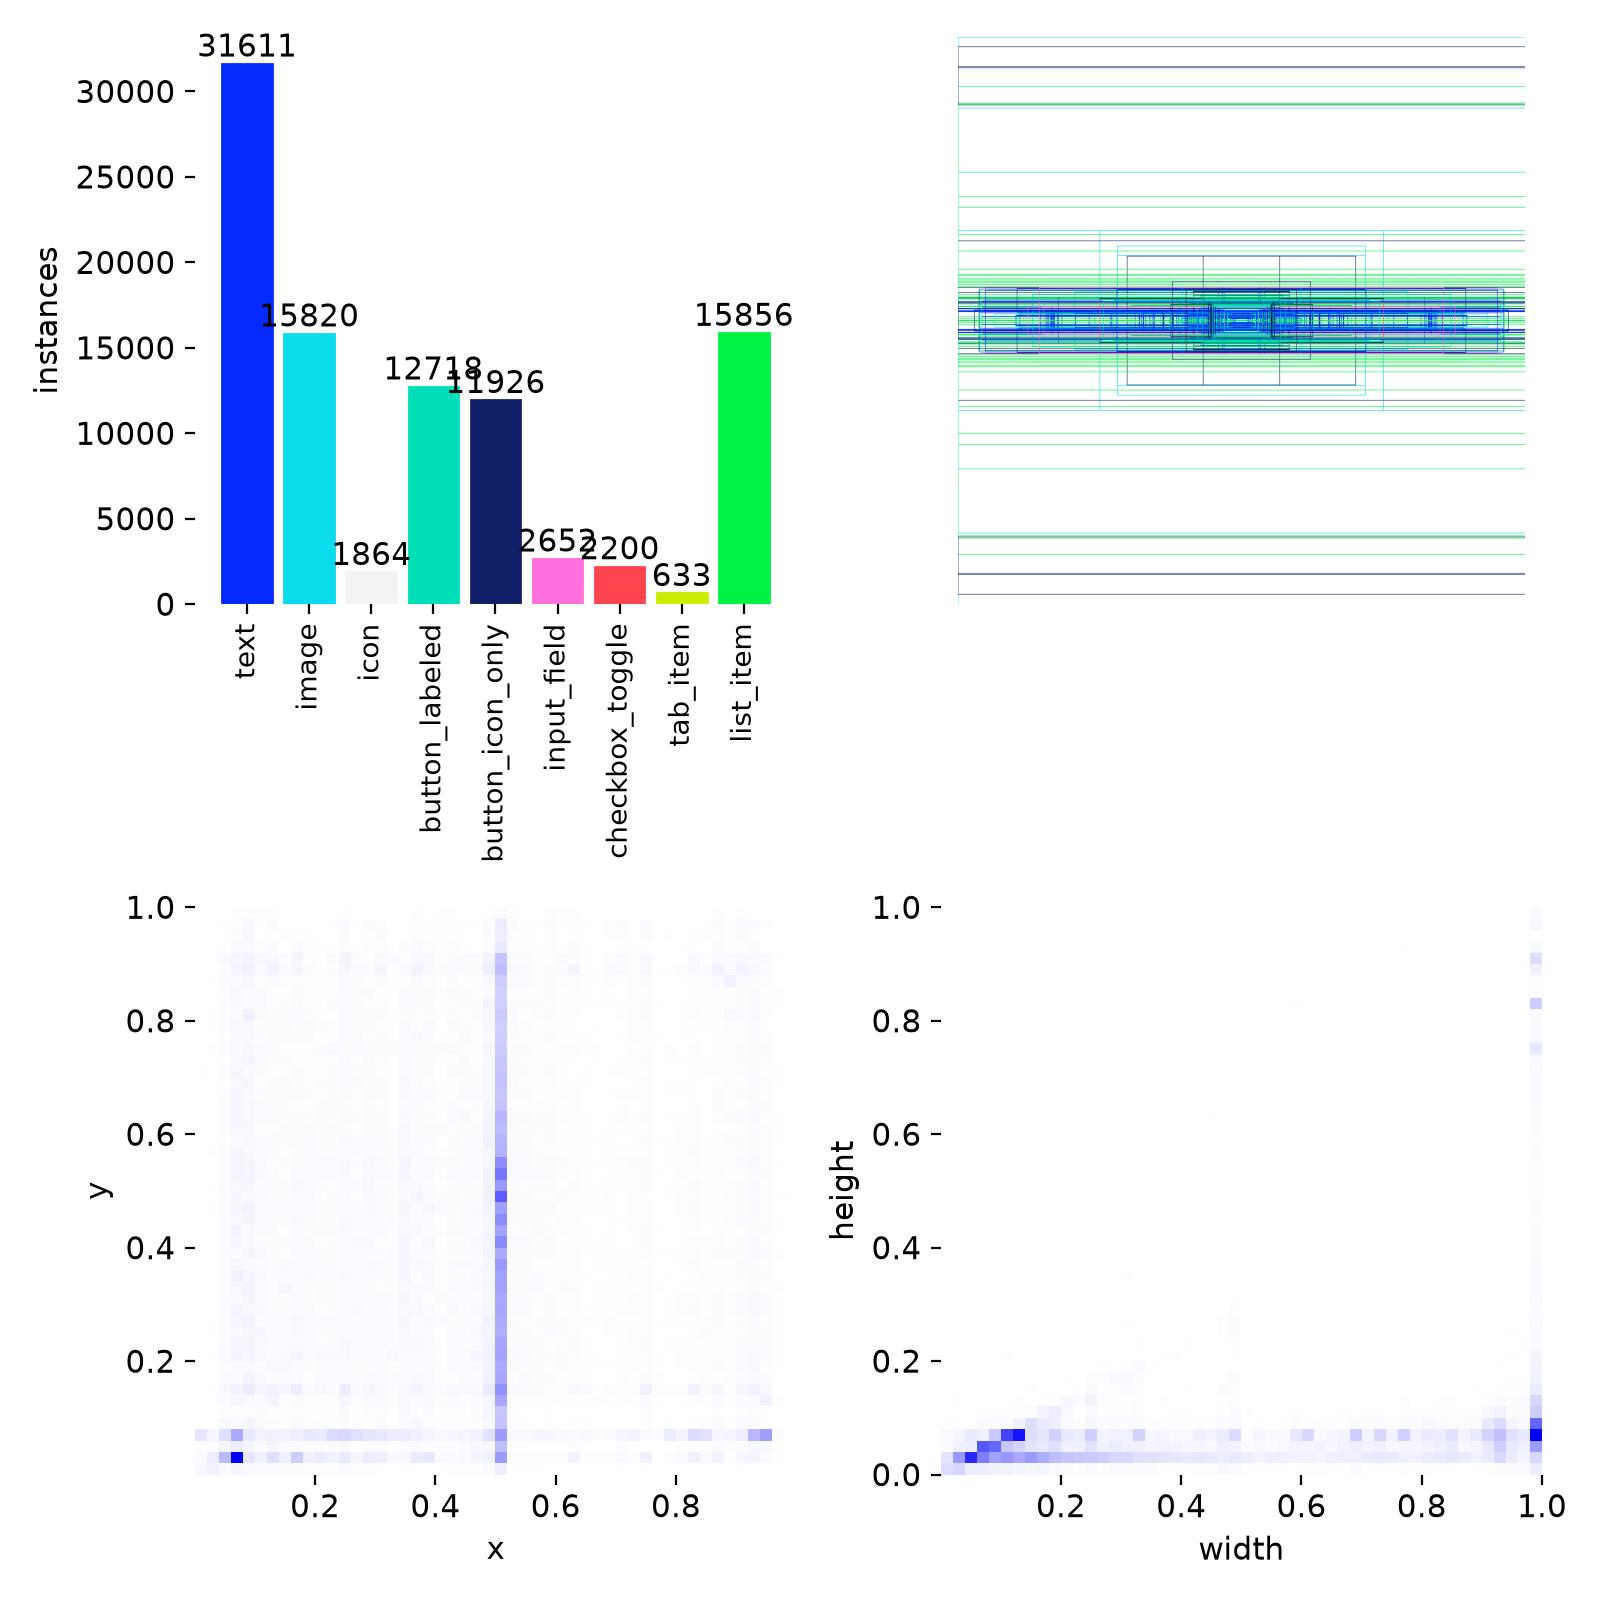
\includegraphics[width=0.55\textwidth]{labels.jpg}
\caption{YOLO11s training-set label statistics: per-class instance counts and the spatial (x,y) and scale (width, height) distribution of ground-truth boxes across the MASC train split, auto-generated by Ultralytics.}
\label{fig:yolo_labels}
\end{figure*}

\begin{figure*}[!t]
\centering
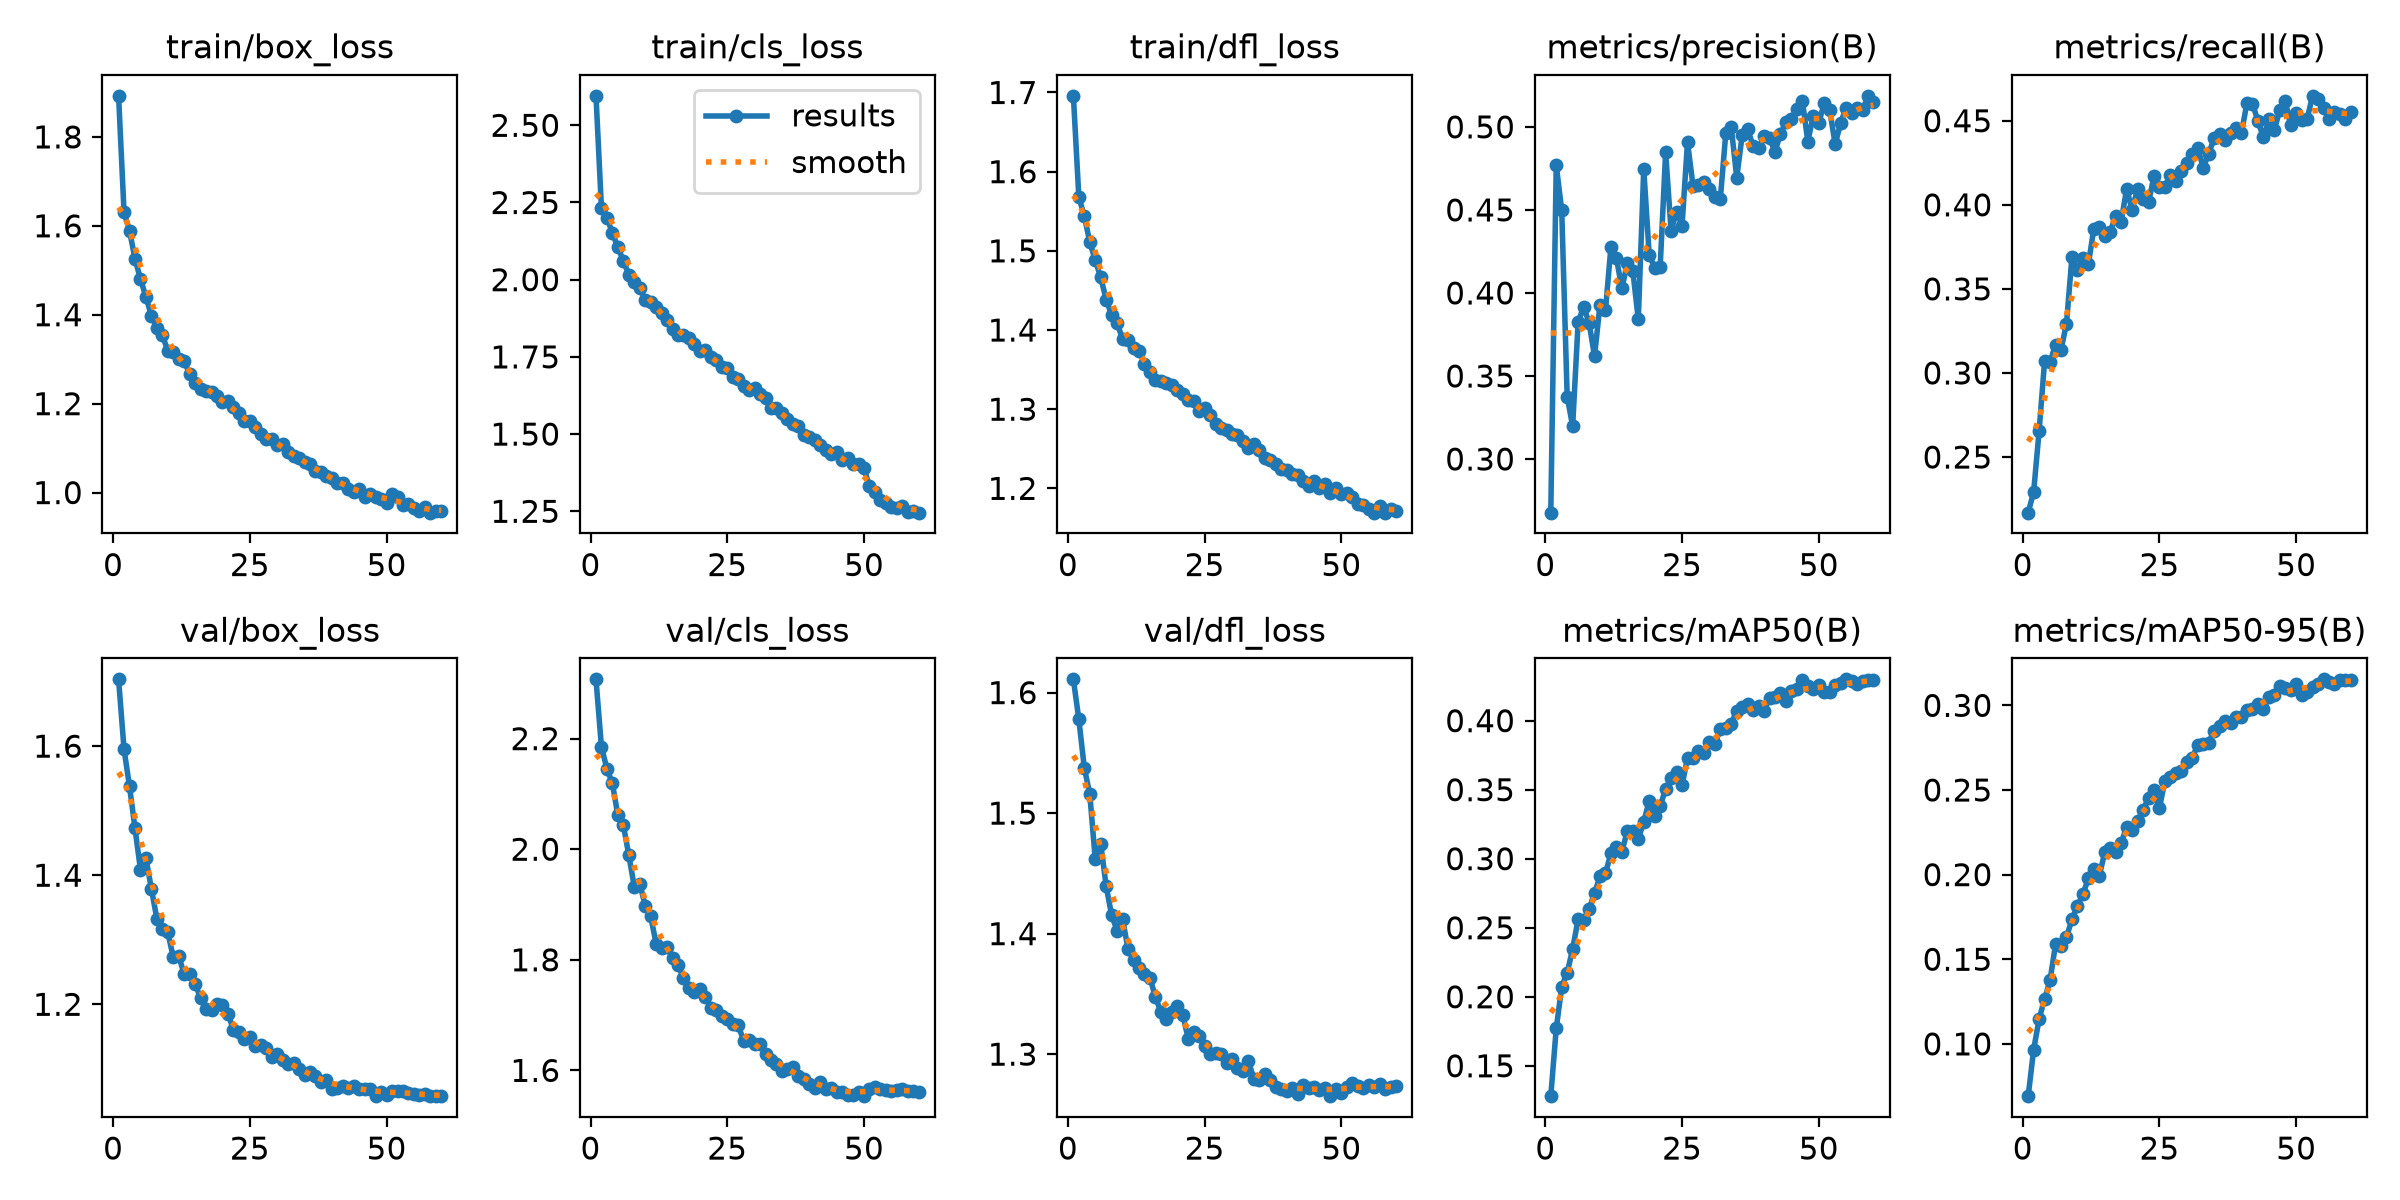
\includegraphics[width=0.92\textwidth]{results.png}
\caption{YOLO11s training run: box/classification/DFL loss and precision/recall/mAP50/mAP50-95 over 60 epochs (train and validation splits), auto-generated by Ultralytics from \texttt{results.csv}.}
\label{fig:yolo_results}
\end{figure*}

\begin{figure*}[!t]
\centering
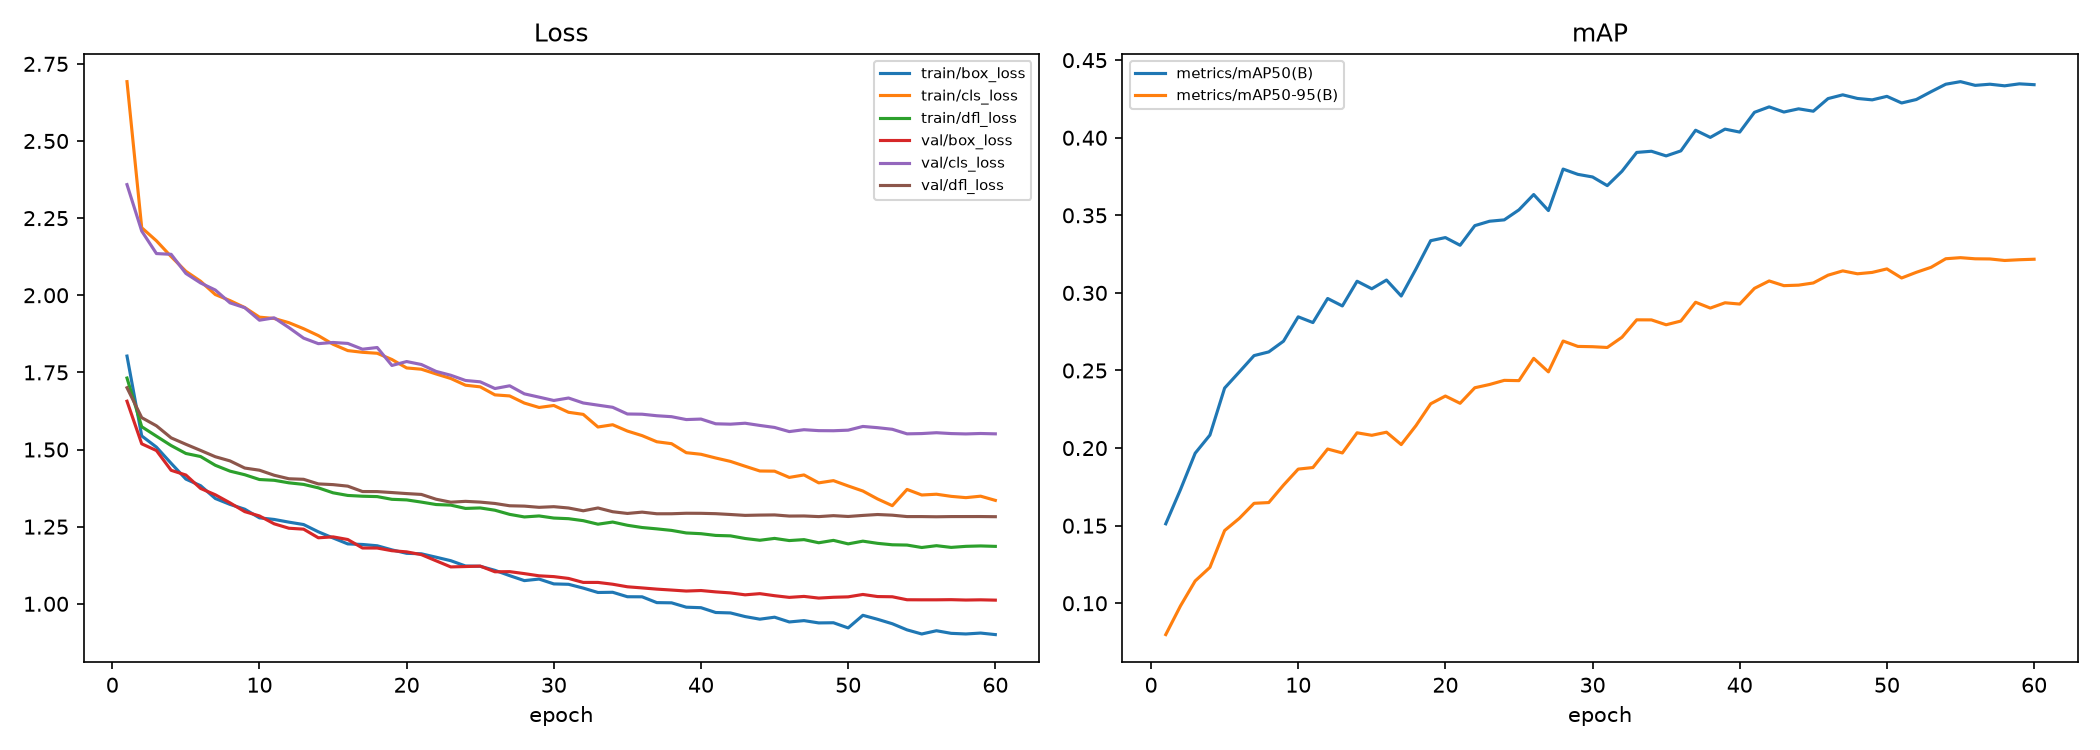
\includegraphics[width=0.85\textwidth]{../../runs/runs/yolo_ui_detector/yolo_training_curves.png}
\caption{YOLO11s detector: custom-rendered loss and mAP progression over the 60-epoch run, generated independently of the Ultralytics auto-report for quick visual sign-off.}
\label{fig:yolo_traincurves}
\end{figure*}

\begin{figure*}[!t]
\centering
\begin{subfigure}[t]{0.48\textwidth}
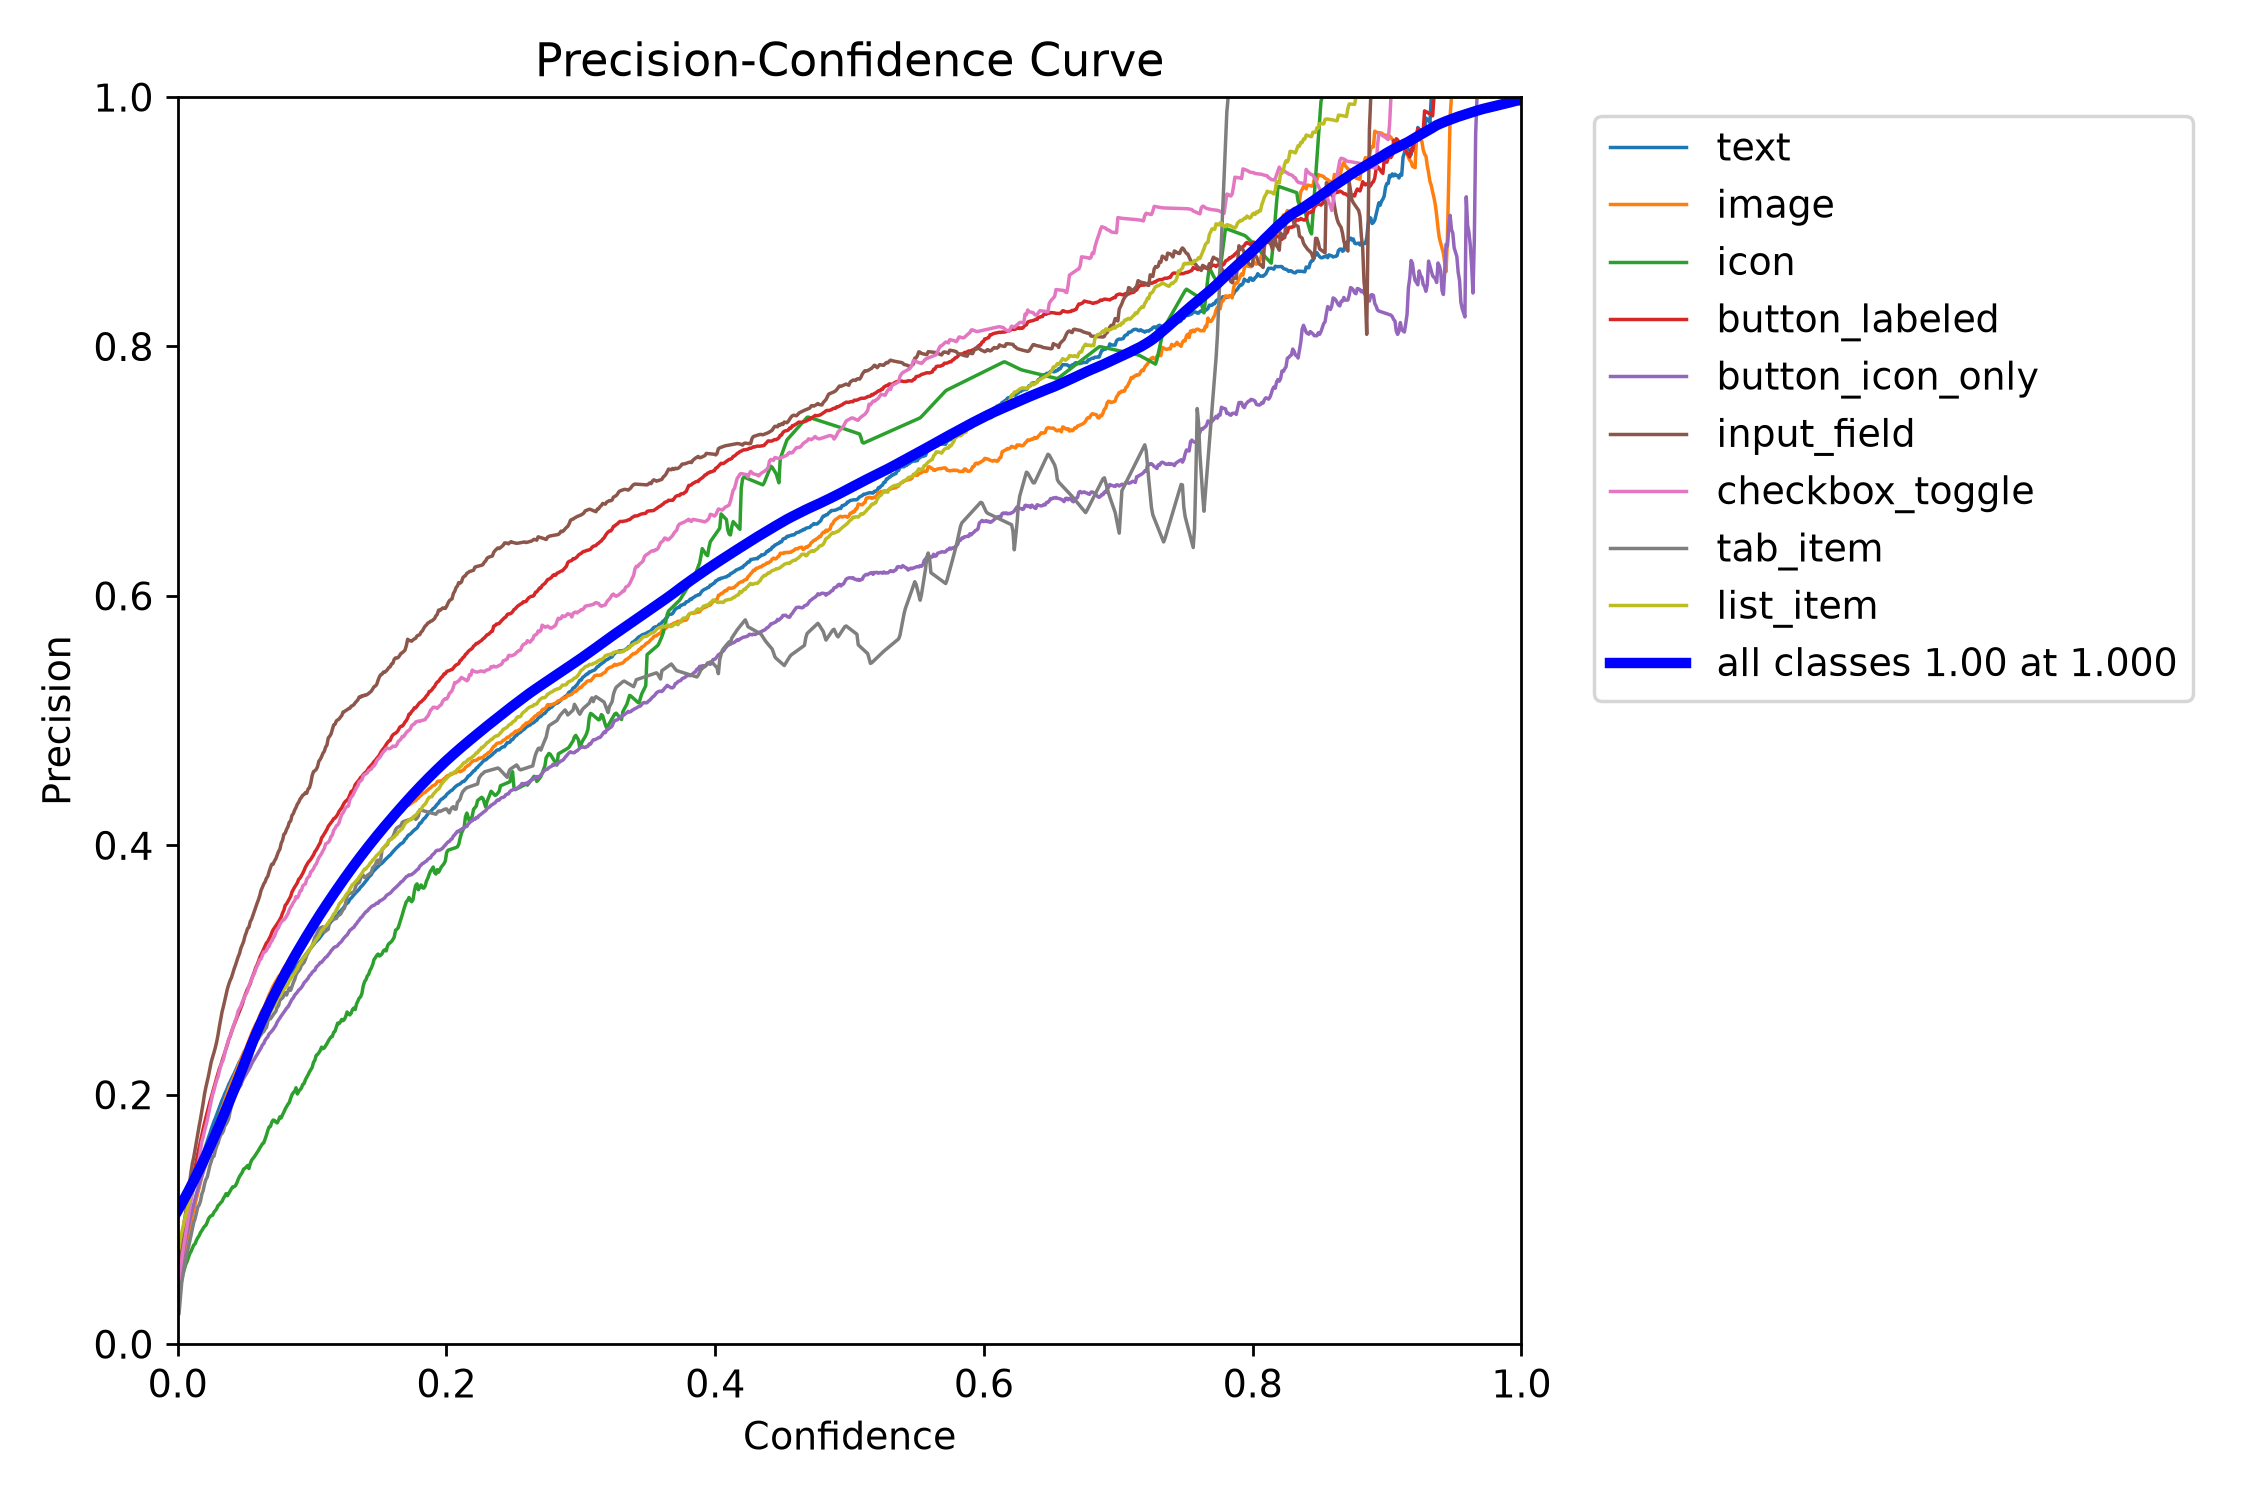
\includegraphics[width=\linewidth]{BoxP_curve.png}
\caption{Precision vs.\ confidence}
\end{subfigure}\hfill
\begin{subfigure}[t]{0.48\textwidth}
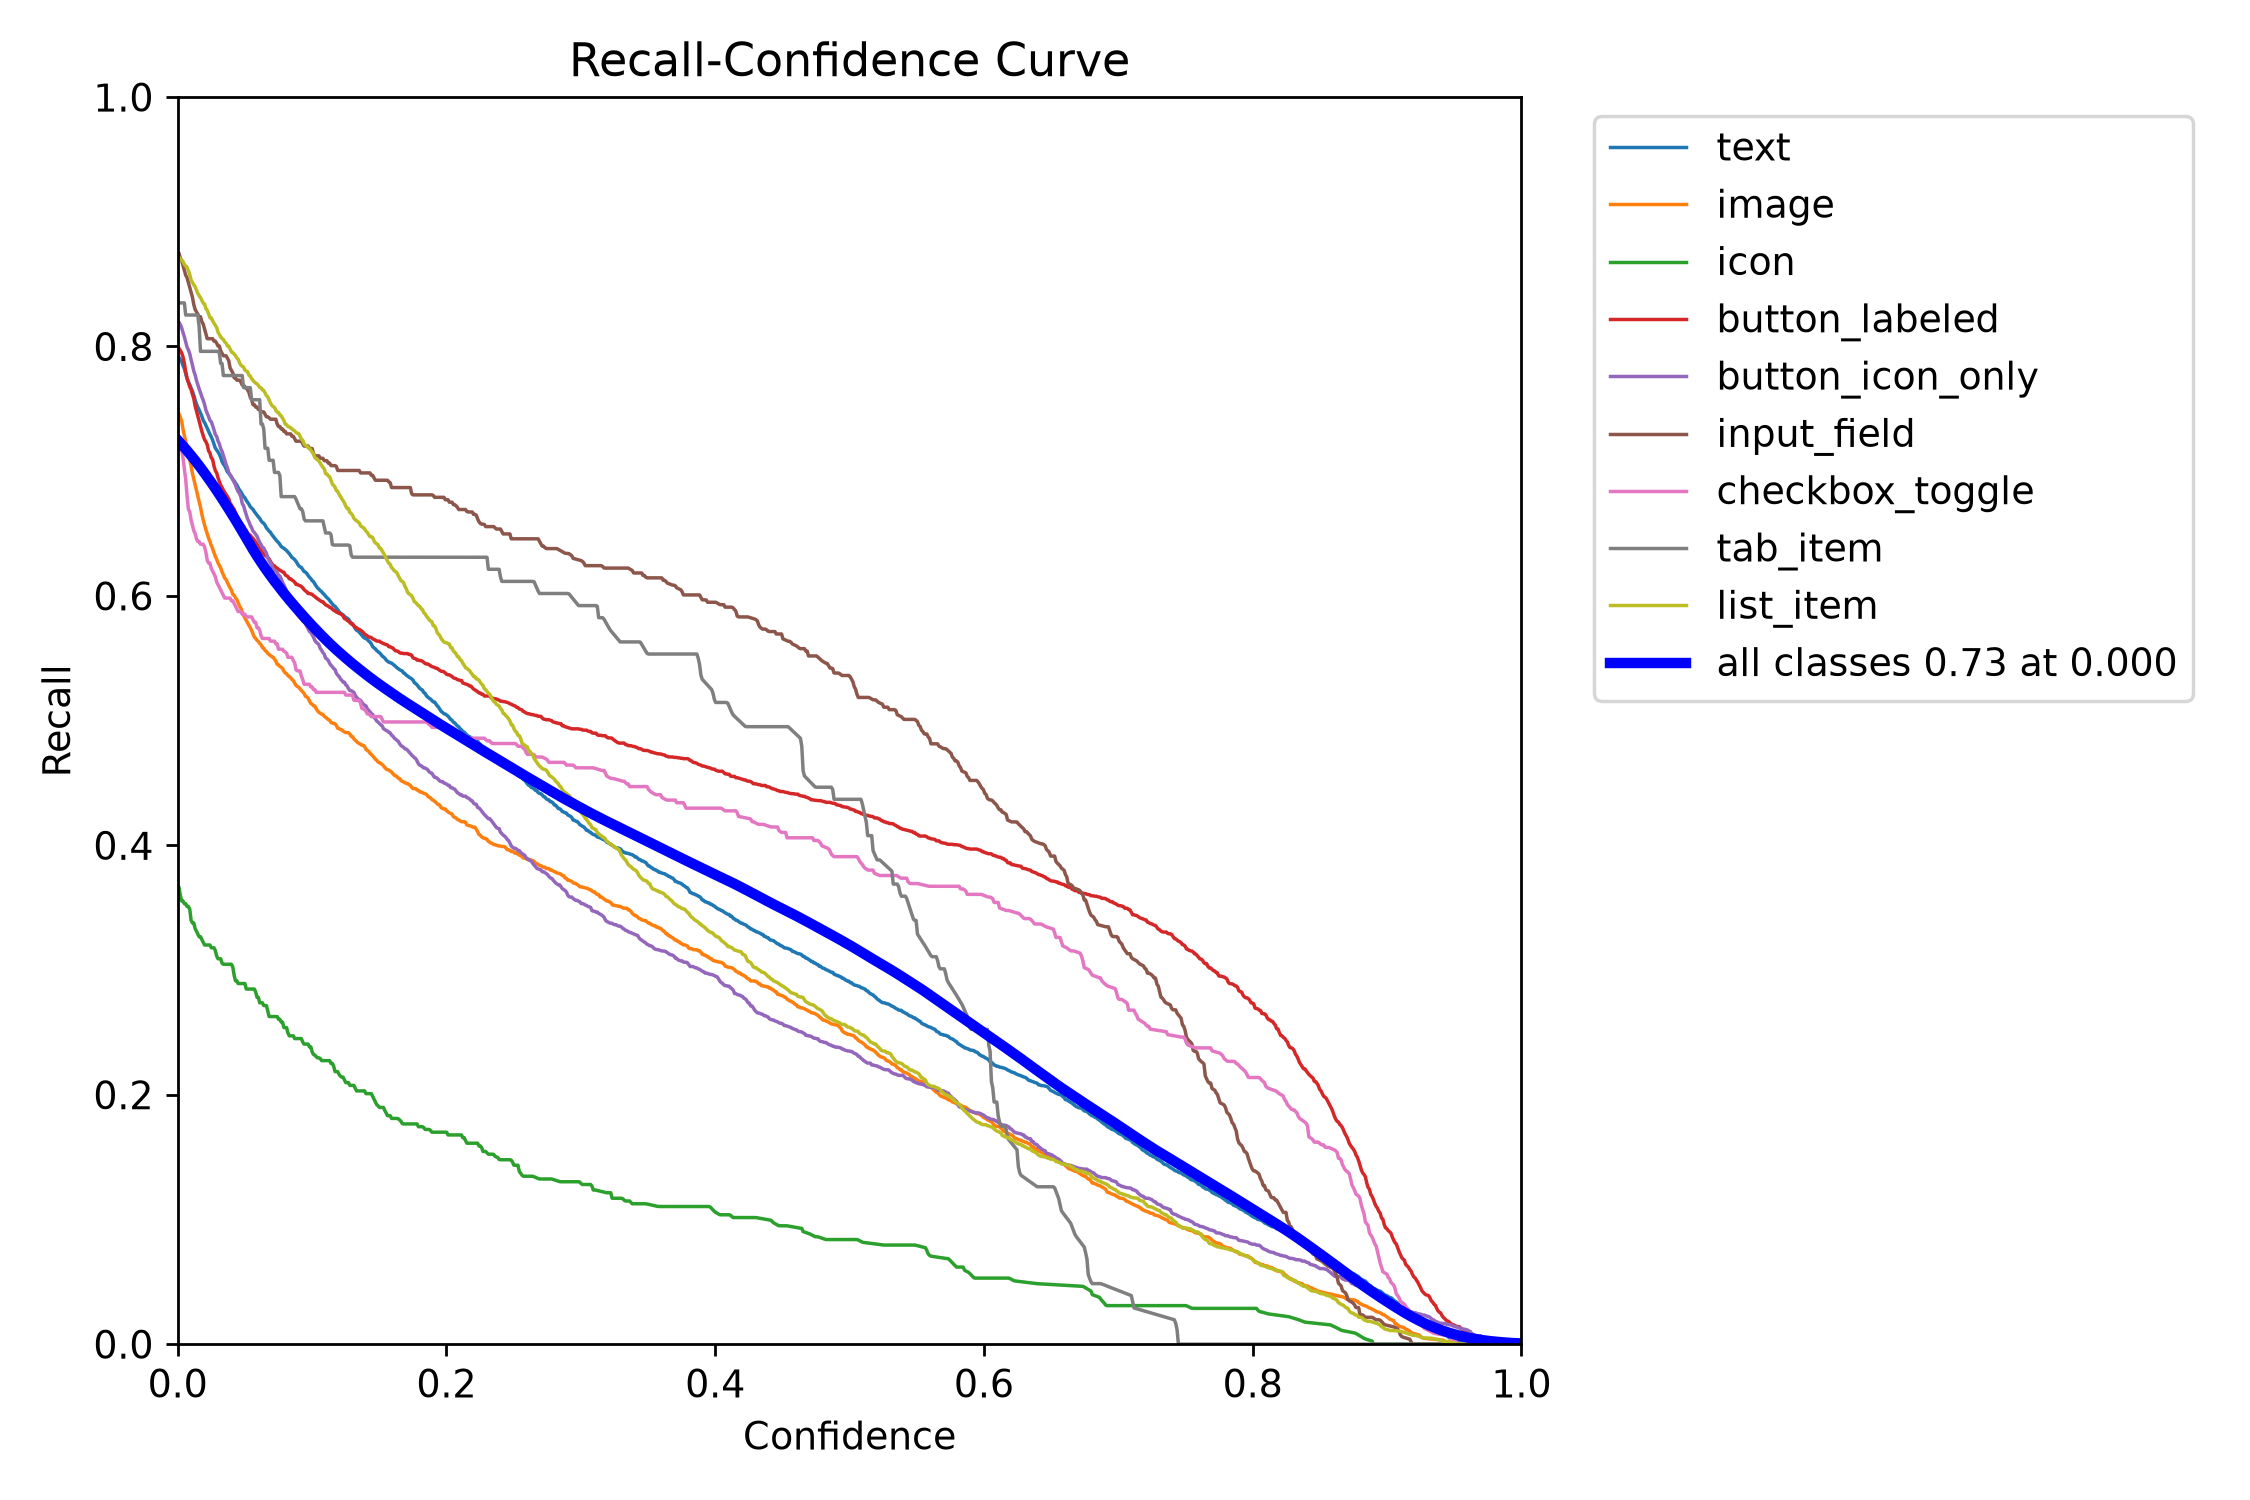
\includegraphics[width=\linewidth]{BoxR_curve.png}
\caption{Recall vs.\ confidence}
\end{subfigure}
\par\smallskip
\begin{subfigure}[t]{0.48\textwidth}
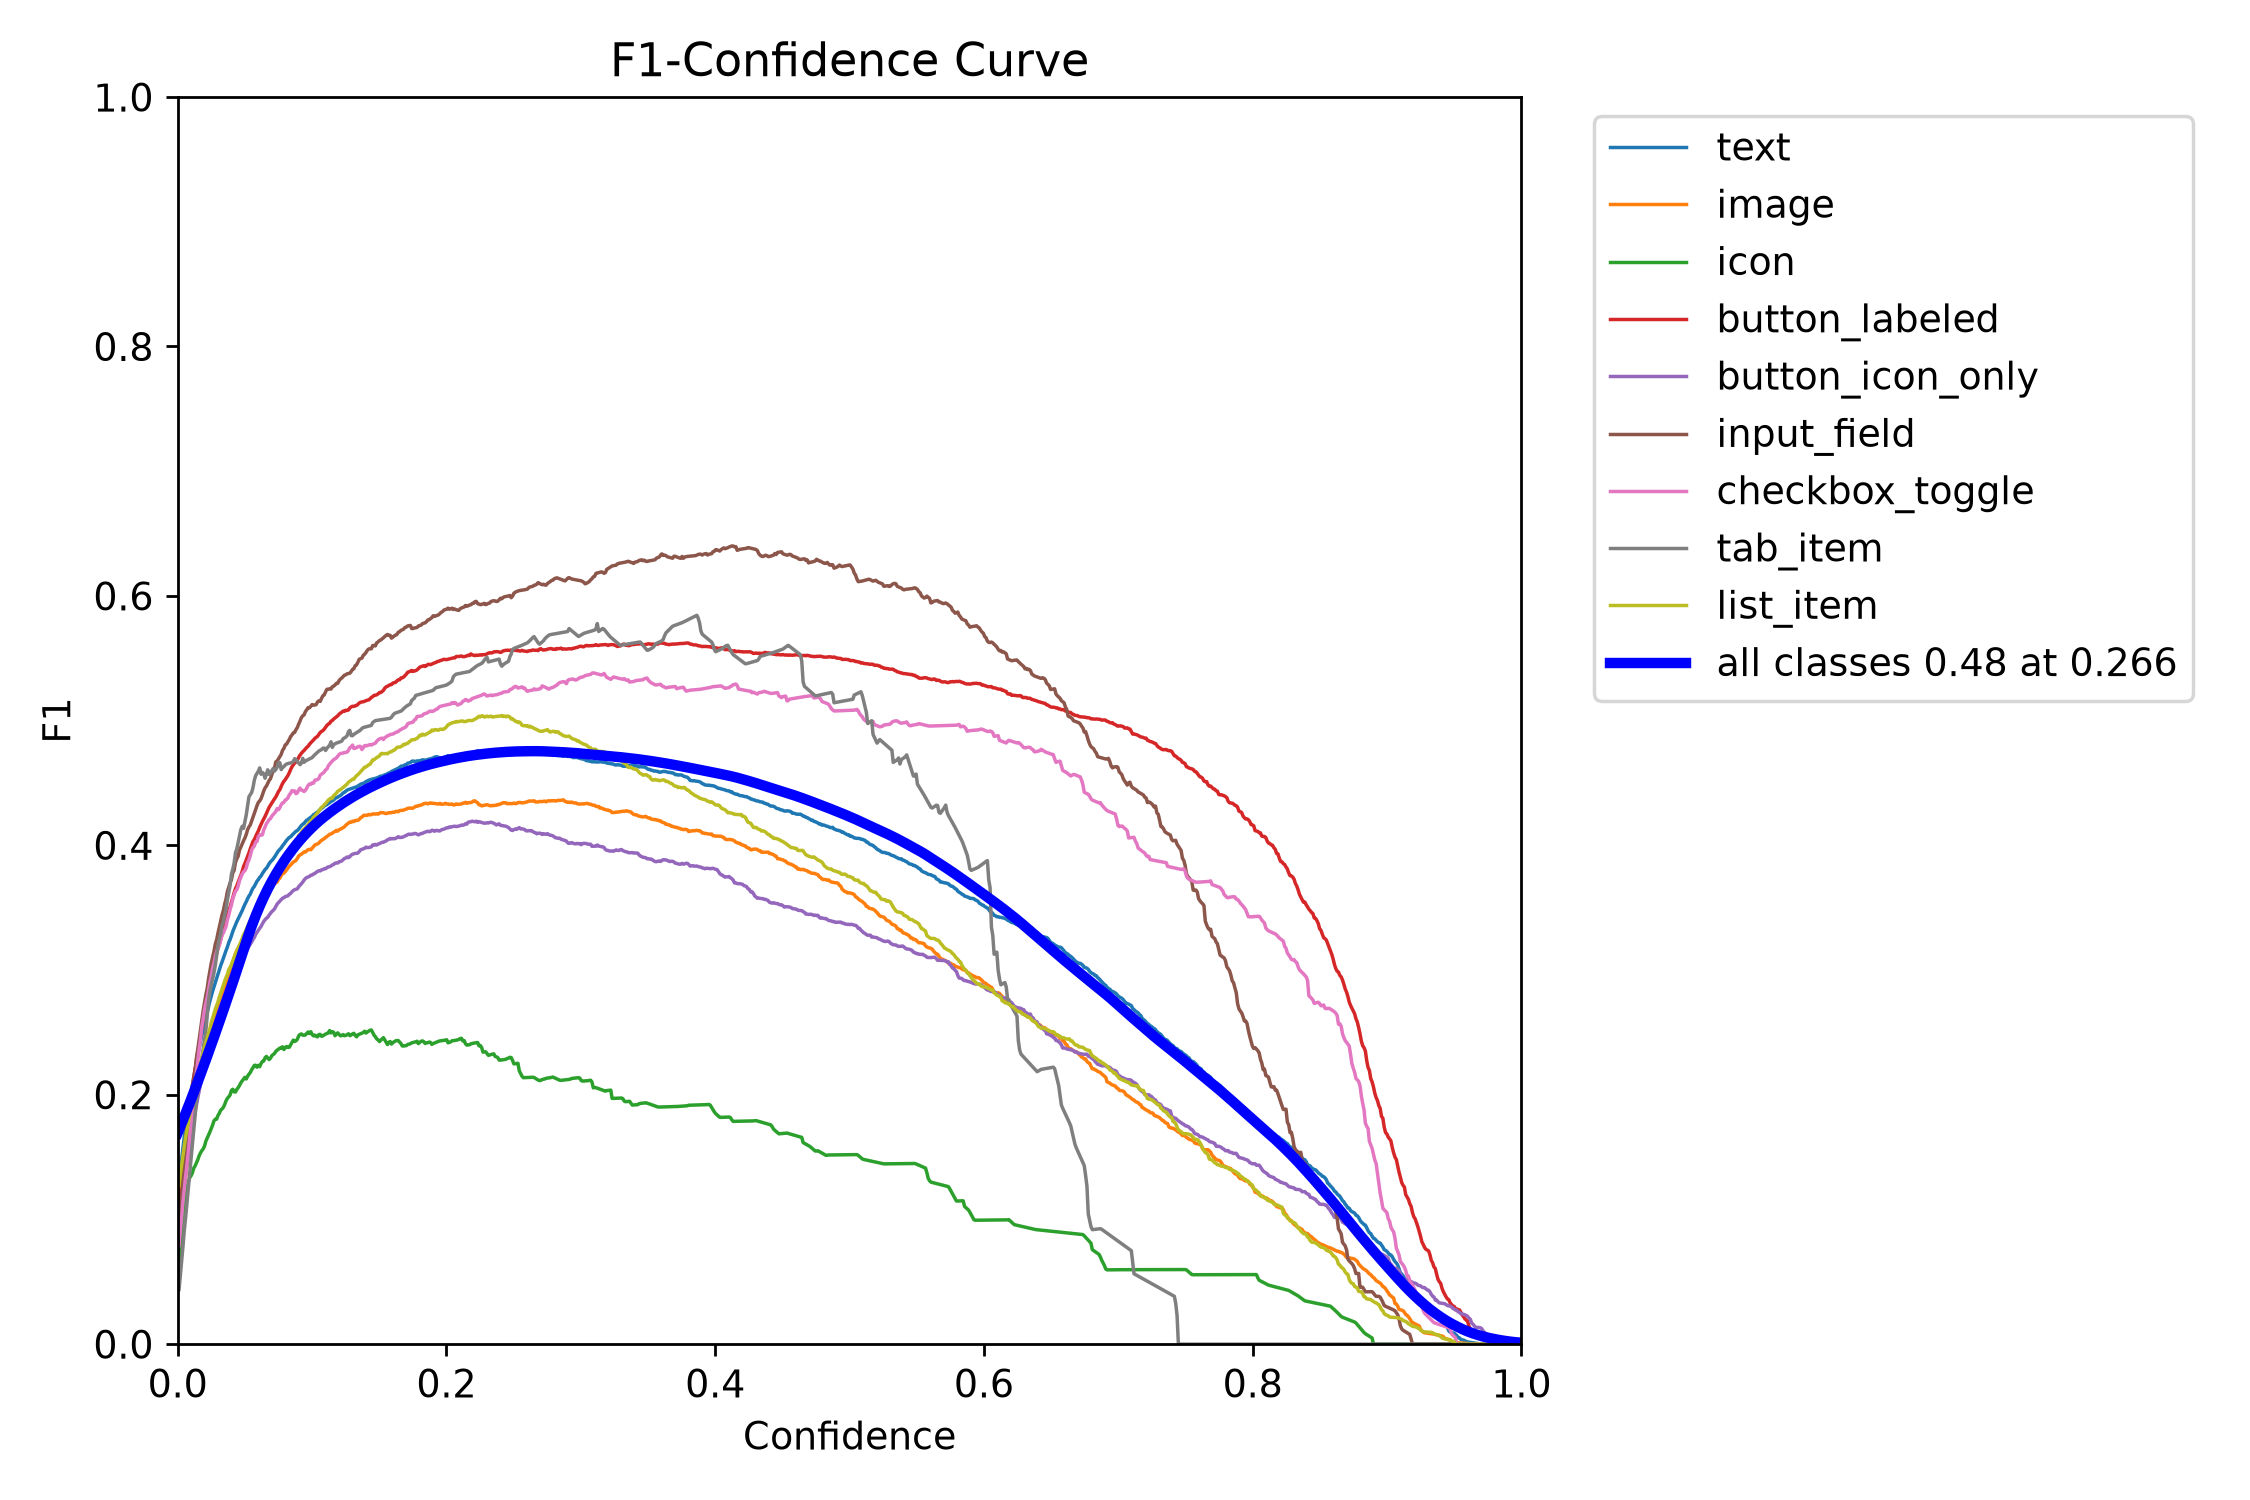
\includegraphics[width=\linewidth]{BoxF1_curve.png}
\caption{F1 vs.\ confidence}
\end{subfigure}\hfill
\begin{subfigure}[t]{0.48\textwidth}
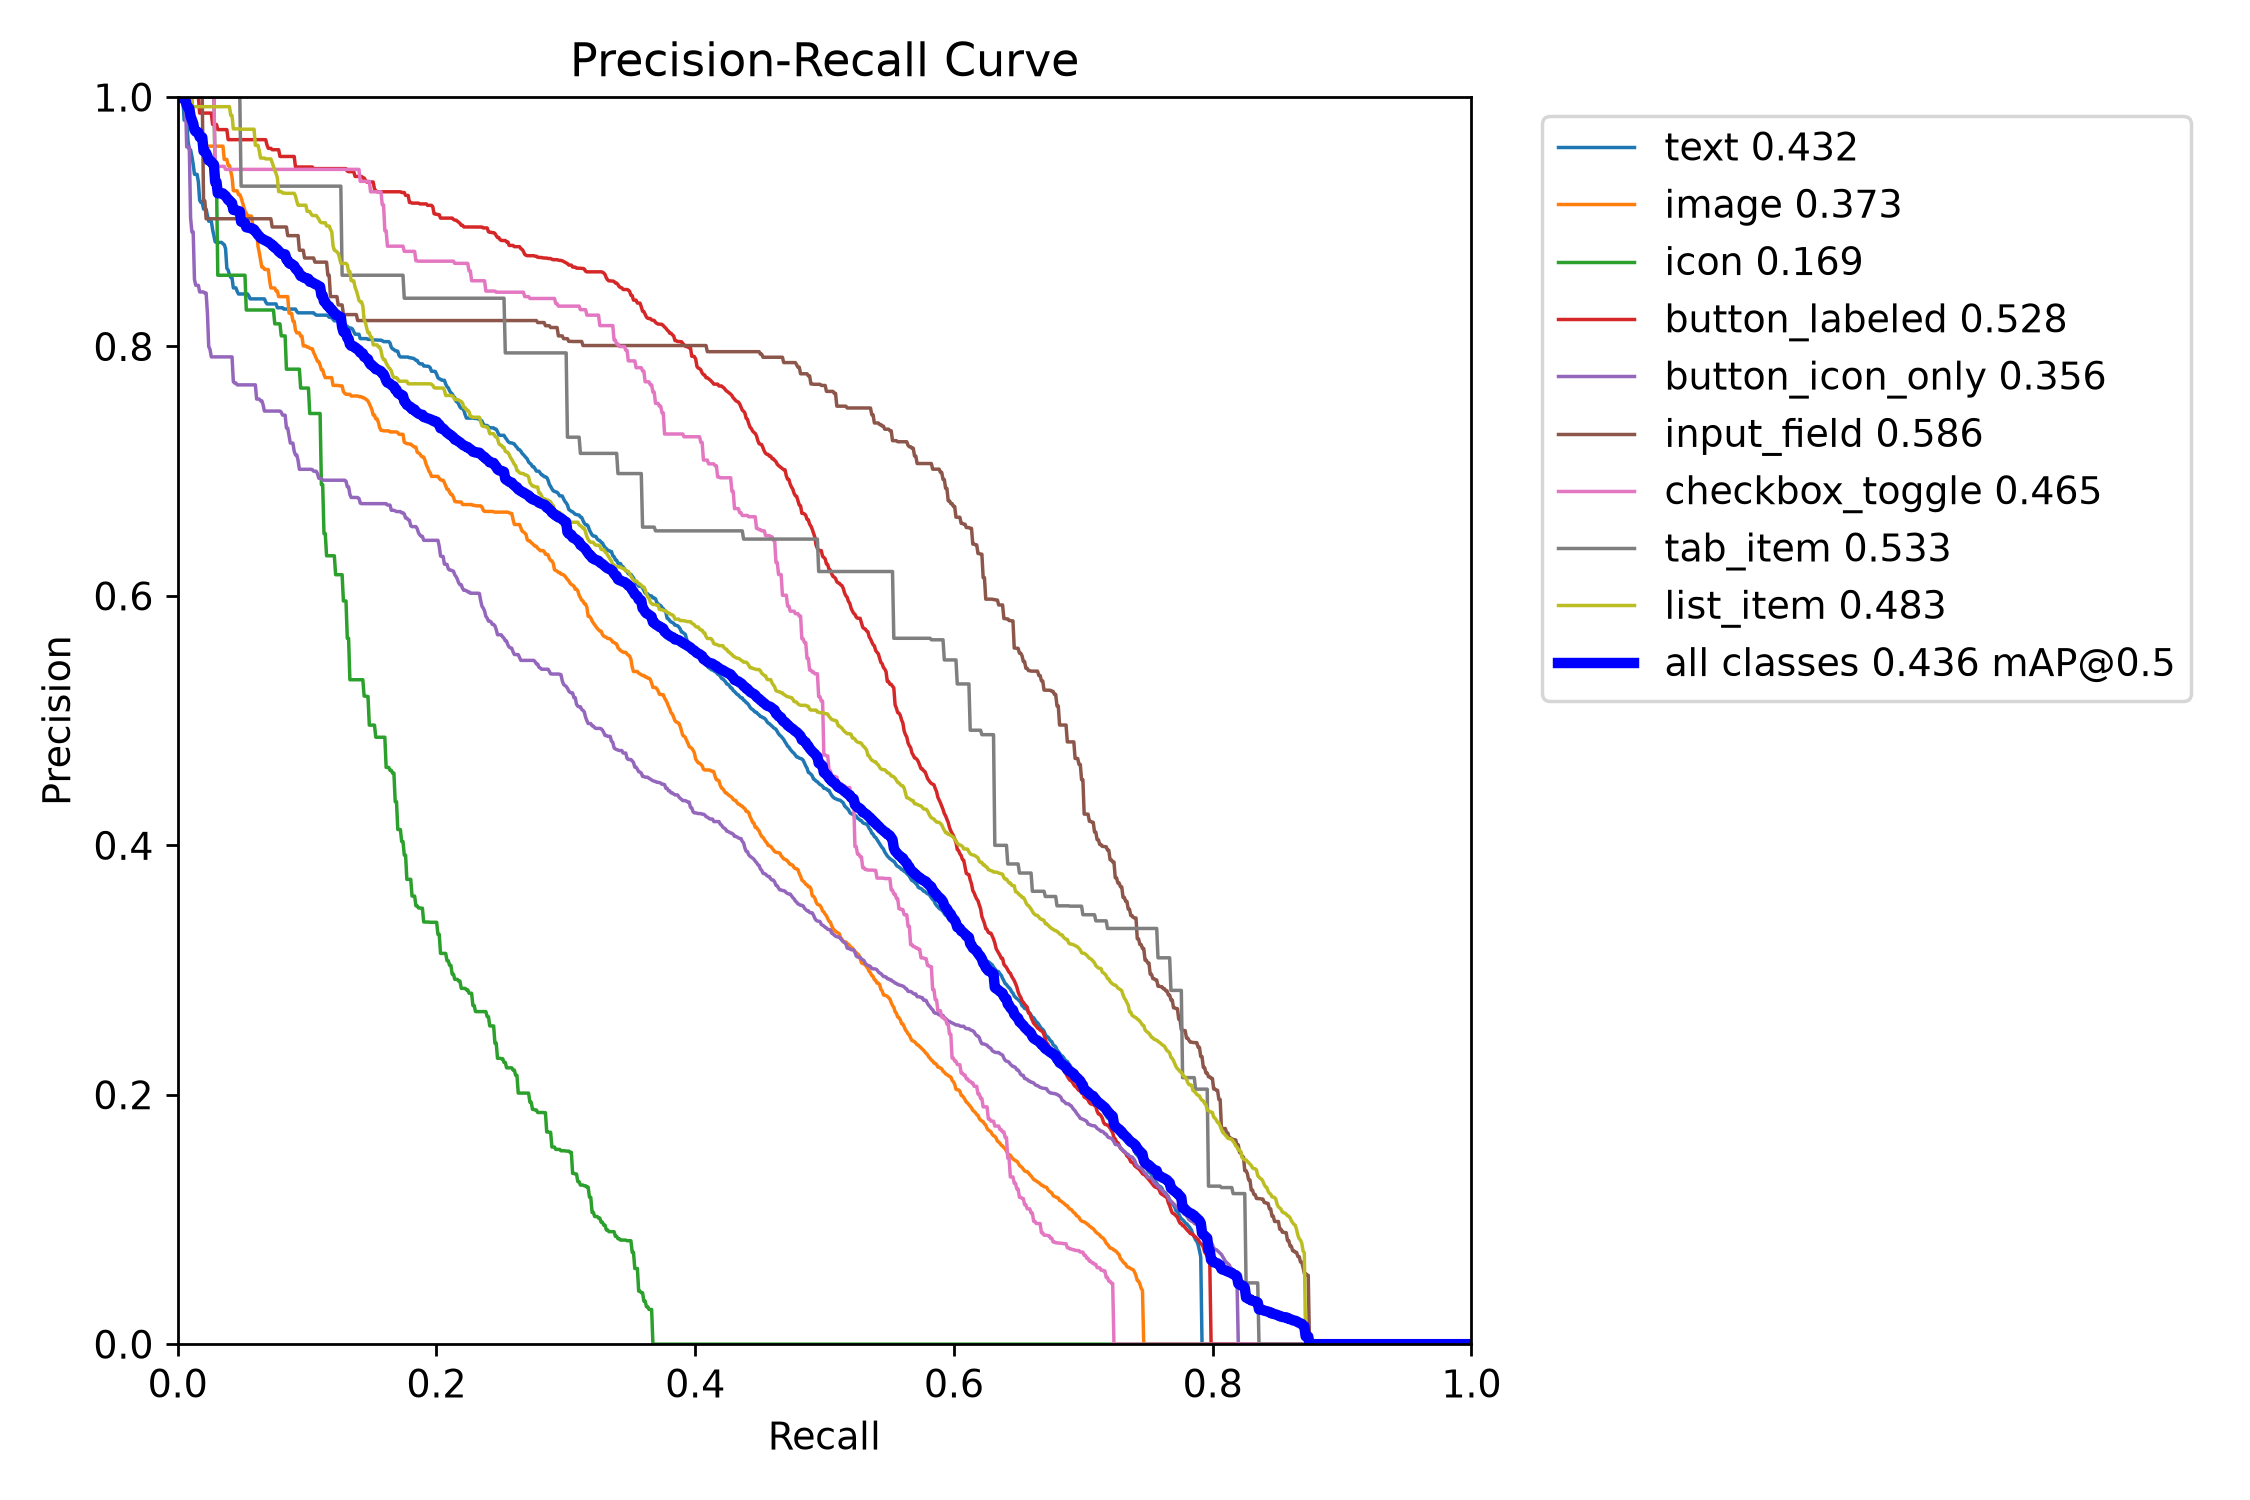
\includegraphics[width=\linewidth]{BoxPR_curve.png}
\caption{Precision--Recall}
\end{subfigure}
\caption{YOLO11s per-class Precision, Recall, F1, and Precision--Recall curves on the MASC validation split.}
\label{fig:yolo_curves}
\end{figure*}

\begin{figure*}[!t]
\centering
\begin{subfigure}[t]{0.48\textwidth}
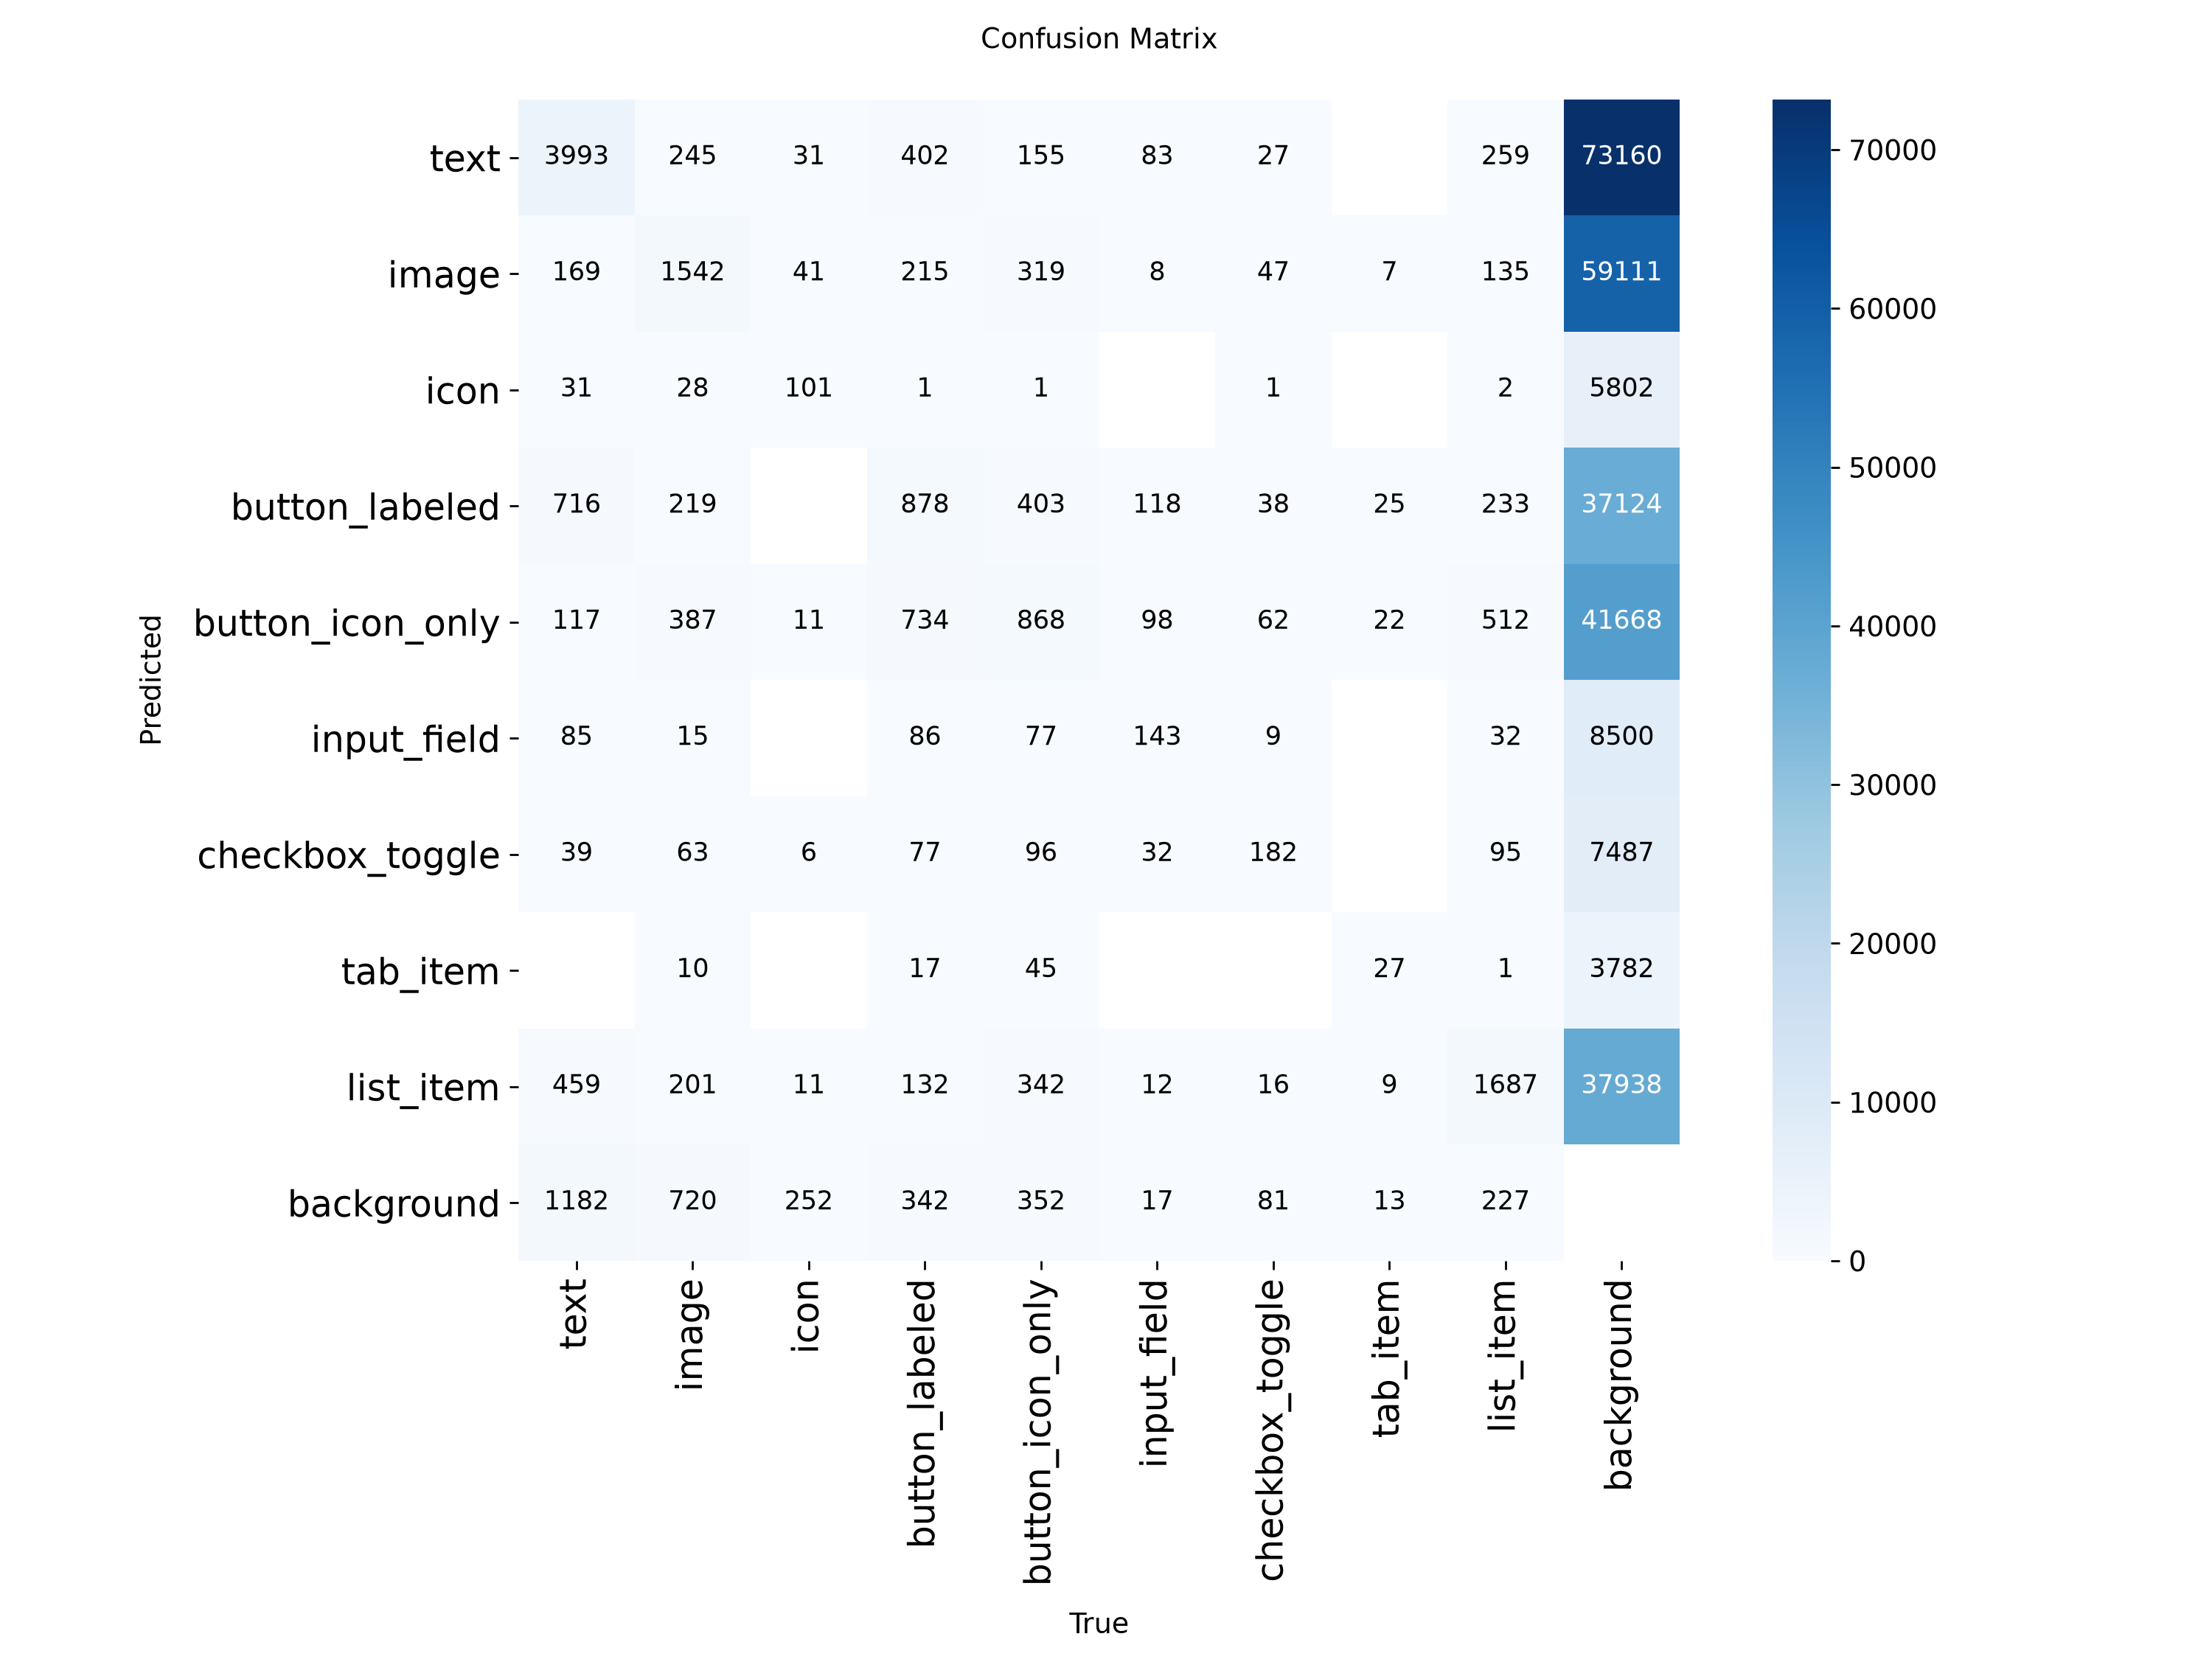
\includegraphics[width=\linewidth]{confusion_matrix.png}
\caption{Raw confusion matrix}
\end{subfigure}\hfill
\begin{subfigure}[t]{0.48\textwidth}
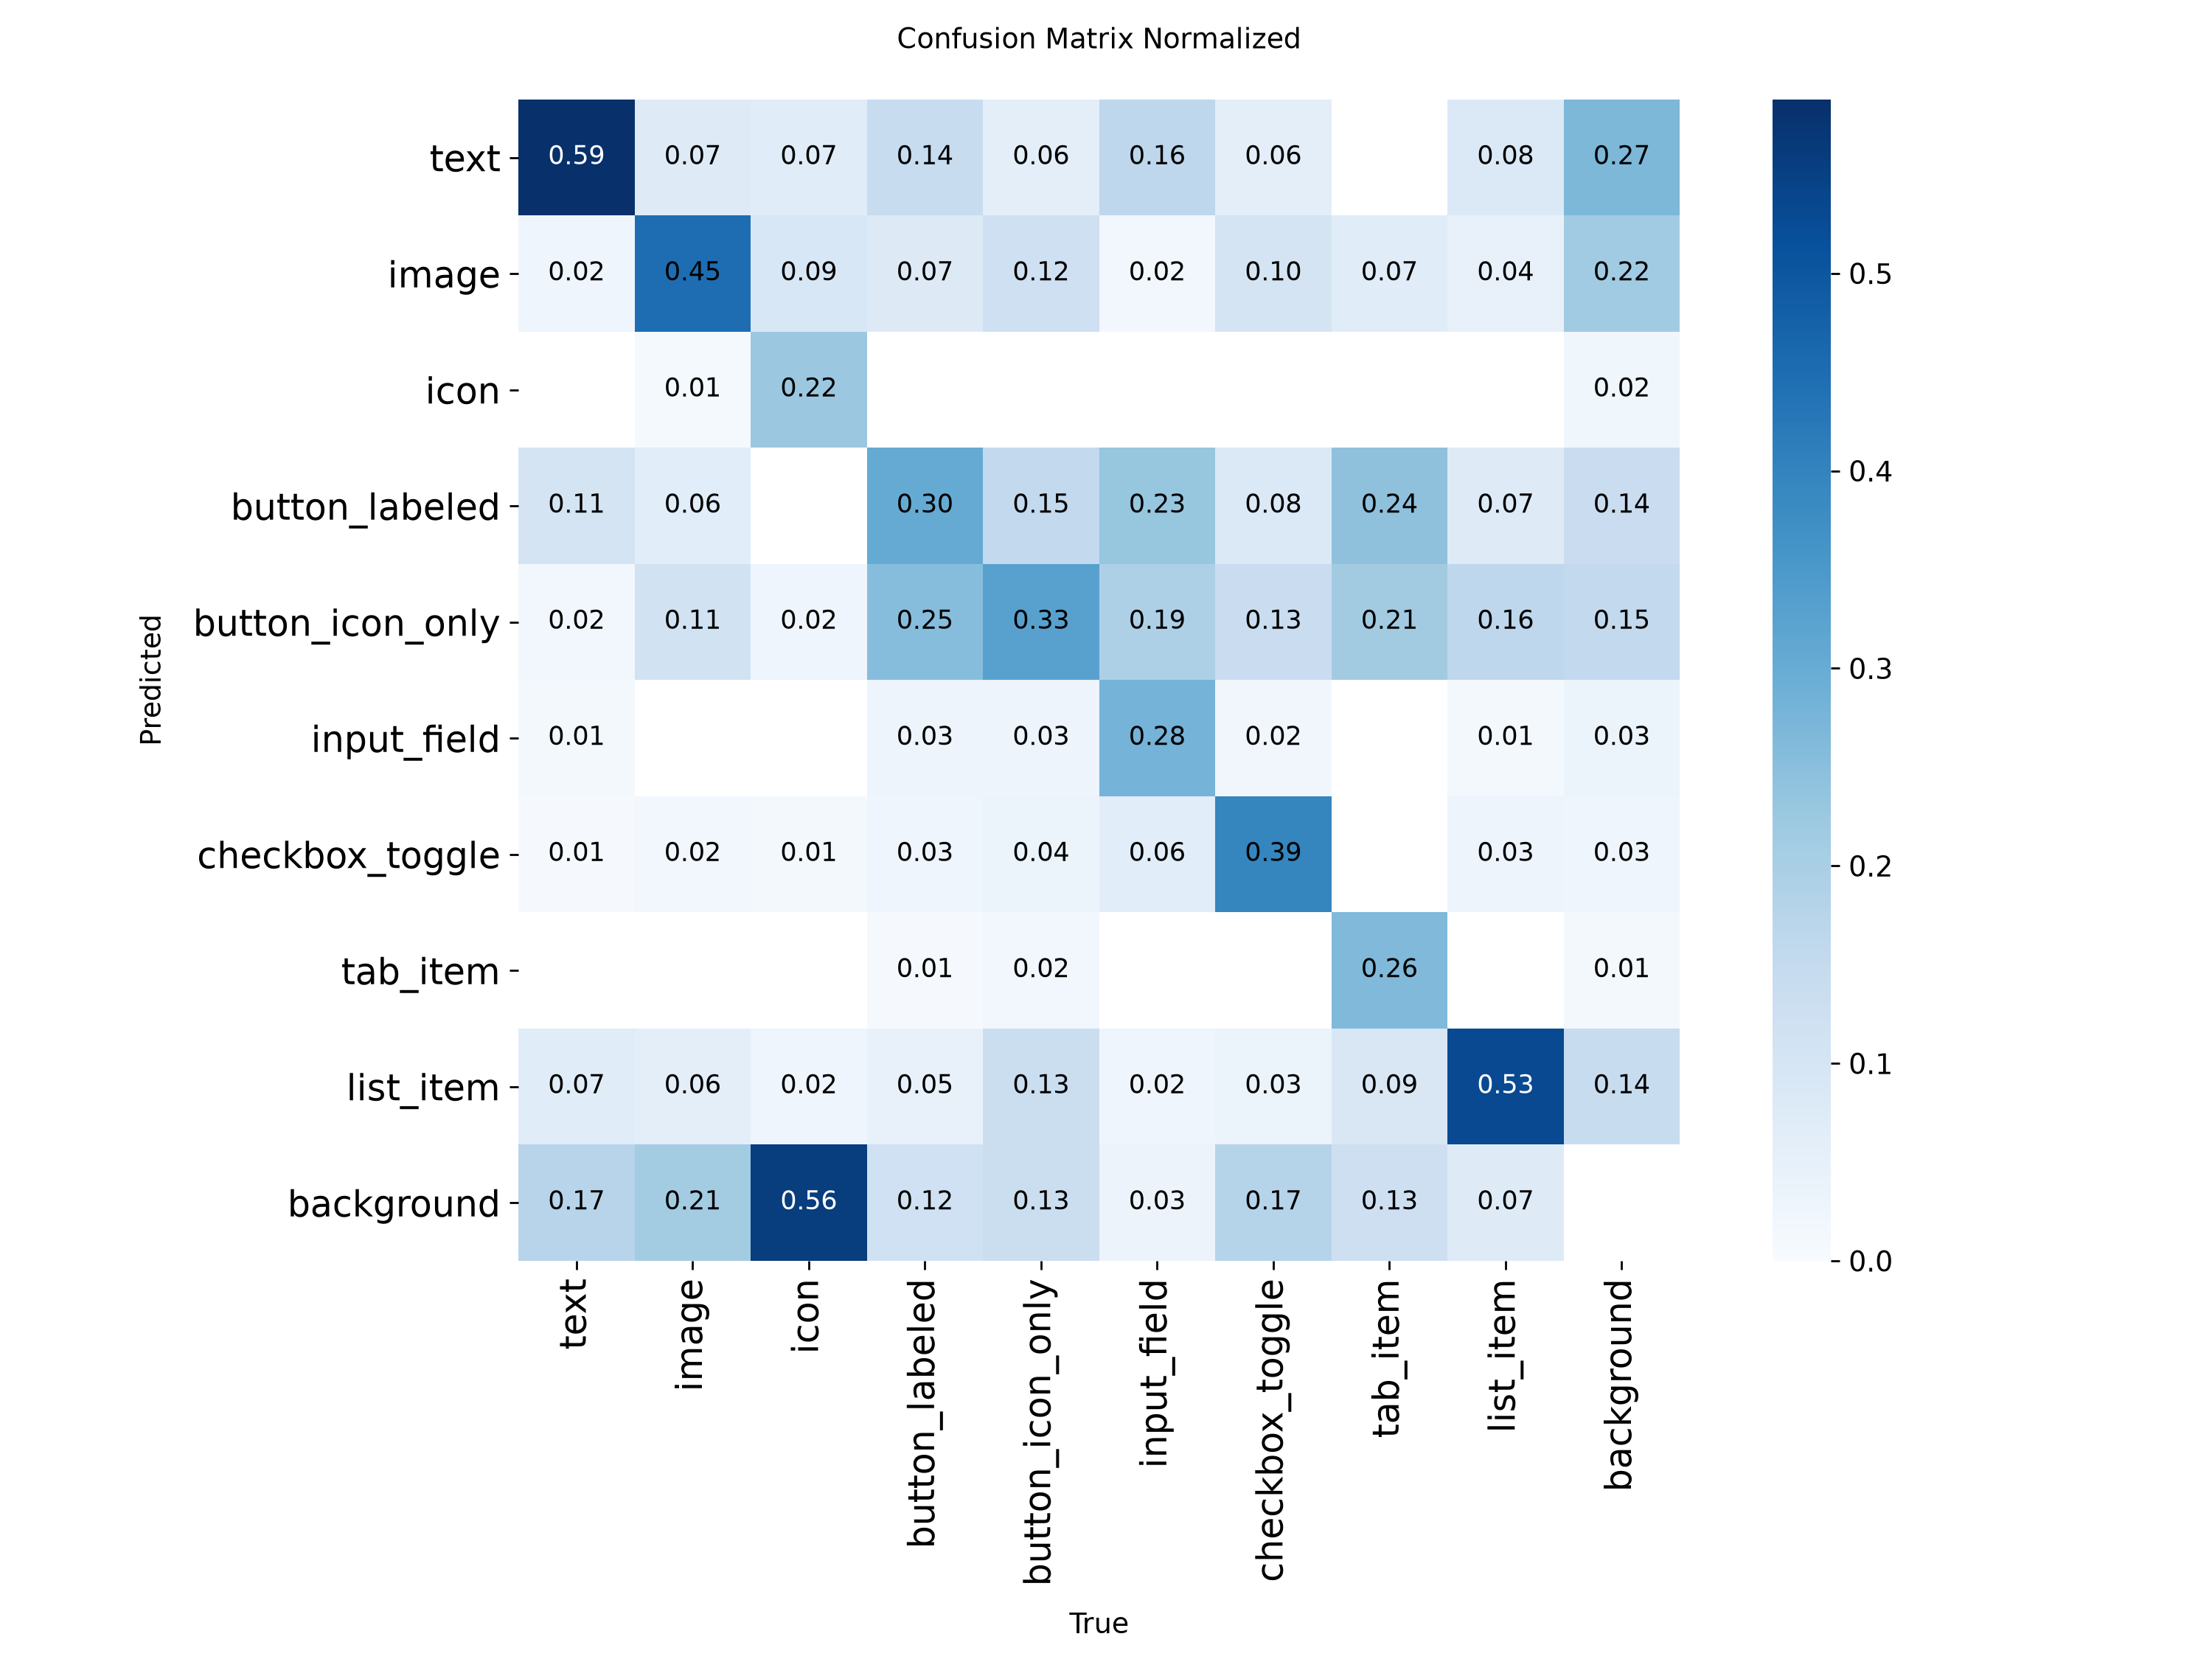
\includegraphics[width=\linewidth]{confusion_matrix_normalized.png}
\caption{Row-normalized confusion matrix}
\end{subfigure}
\caption{YOLO11s confusion matrices across the 9-class UI-element taxonomy plus background, MASC validation split.}
\label{fig:yolo_cm}
\end{figure*}

Table~\ref{tab:yolo} summarizes the final 60-epoch results on the MASC validation split alongside the Rico holdout generalization check.

\begin{table}[!t]
\caption{YOLO11s UI-element detector results.}
\label{tab:yolo}
\centering
\scriptsize
\begin{tabular}{@{}lrr@{}}
\toprule
\textbf{Metric} & \textbf{MASC val (epoch 60)} & \\
\midrule
Precision & 0.535 & \\
Recall & 0.447 & \\
mAP50 & 0.434 & \\
mAP50-95 & 0.322 & \\
\midrule
\textbf{Rico holdout (unseen)} & \textbf{Zero-shot} & \textbf{Fine-tuned} \\
mAP50 & 0.0258 & 0.2546 \\
mAP50-95 & 0.0116 & 0.1732 \\
\bottomrule
\end{tabular}
\end{table}

Fine-tuning yields roughly a $10\times$ lift in mAP50 over the untrained base model on apps never seen during training, confirming that the training signal transfers beyond MASC, although absolute accuracy on unseen layouts (mAP50 $\approx$0.25) remains moderate. The detector is wired into \texttt{backend/routers/audit.py}: the \texttt{xml} field on \texttt{POST /api/v1/audit} is optional, and \texttt{\_run\_pipeline} falls back to \texttt{detect\_ui()} on missing, malformed, or empty-hierarchy XML. Figures~\ref{fig:cv-waiting} and \ref{fig:cv-ready} show the Axion Upload screen states that surface this fallback path to the user.

\begin{figure}[!t]
\centering
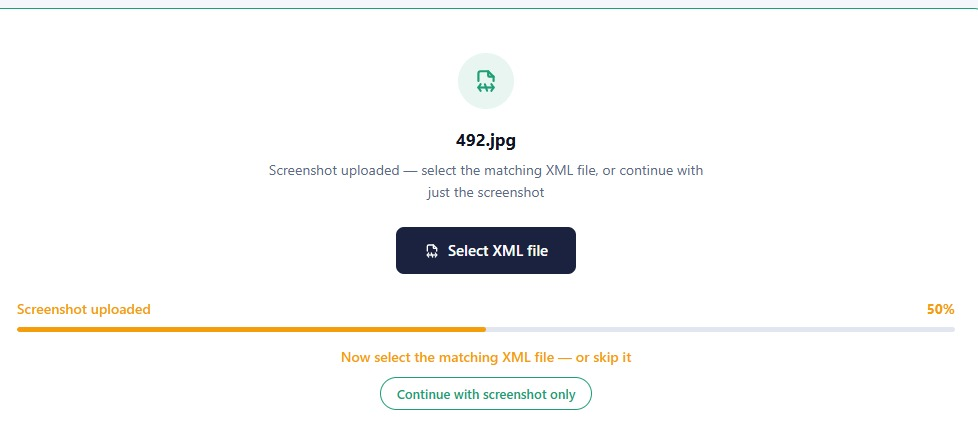
\includegraphics[width=\linewidth]{figma-09-screenshot-only-waiting.jpg}
\caption{Axion Upload: screenshot-only mode, awaiting the YOLO fallback detector while no XML is supplied.}
\label{fig:cv-waiting}
\end{figure}

\begin{figure}[!t]
\centering
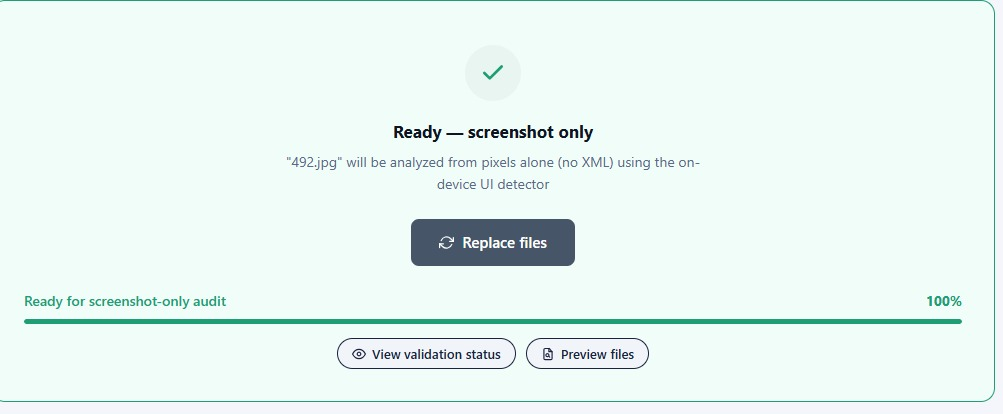
\includegraphics[width=\linewidth]{figma-10-screenshot-only-ready.jpg}
\caption{Axion Upload: screenshot-only audit ready to start once pixel-based detection completes.}
\label{fig:cv-ready}
\end{figure}

\subsubsection{Multi-Label Crop-Violation Classifier}
Six of the thirty rules (R09 contrast, R04 touch-target size, R17 spacing, R10 text overflow, R28 font-scale overflow, R08 layout overlap) describe properties that only fully exist once a layout is \emph{rendered} -- bounds math from the XML alone can approximate but not confirm them. \texttt{src/crop\_violation\_classifier.py} implements a multi-label image classifier -- since one crop can trigger more than one rule simultaneously, e.g., a control that is both too small and too close to its neighbor -- that predicts a subset of $\{$R09, R04, R17, R10, R28, R08$\}$ for a 224$\times$224 crop of a screenshot region. Positive/negative crop labels are generated by re-running the already-tested rule checker itself on each MASC screen and keeping only the six target rules, avoiding a re-implementation of contrast/overlap/spacing math. Figure~\ref{fig:crop-samples} shows representative crops from the training set together with qualitative predictions on the MASC test split and the Rico holdout.

\begin{figure*}[!t]
\centering
\begin{subfigure}[t]{0.32\textwidth}

\includegraphics[width=\linewidth]{sample_training_crops.png}
\caption{Training crops}
\end{subfigure}\hfill
\begin{subfigure}[t]{0.32\textwidth}

\includegraphics[width=\linewidth]{sample_test_predictions.png}
\caption{MASC test predictions}
\end{subfigure}\hfill
\begin{subfigure}[t]{0.32\textwidth}

\includegraphics[width=\linewidth]{sample_rico_predictions.png}
\caption{Rico holdout predictions}
\end{subfigure}
\caption{Crop-violation classifier: sample positive/negative training crops, and qualitative multi-label predictions on unseen MASC test and Rico holdout screens.}
\label{fig:crop-samples}
\end{figure*}

Training uses a two-phase fine-tuning schedule (frozen-backbone head-only for epochs 1--3, full unfreeze at a lower learning rate from epoch 4), a \texttt{BCEWithLogitsLoss} with per-rule positive-class weighting capped at 20.0 to counter severe class imbalance, and early stopping on validation macro-F1 (patience 5). The original backbone choice, \texttt{mobilenet\_v3\_small}, was selected early for its low capacity relative to the available dataset size, but that assumption was never empirically tested until a controlled 33-backbone comparison sweep was run against both the MASC test split and the full Rico holdout. The sweep found the original pick mid-pack (Rico macro-F1 0.18, beaten by ten or more candidates), and that attention-based architectures -- not simply modern CNN design tricks -- were driving the gap: a \texttt{convnext\_tiny} control sharing the same design tricks (LayerNorm, patchify stem, inverted bottlenecks) but no attention landed back at pack level (0.18), while \texttt{vit\_b\_16} (global self-attention), \texttt{mobilevitv2\_200} (hybrid CNN/self-attention), and \texttt{swin\_tiny\_patch4\_window7\_224} (windowed/hierarchical self-attention) all scored higher, with Swin-Tiny winning outright at roughly a third of ViT-B/16's parameter count and a more evenly distributed per-rule profile. The backbone was consequently changed to \texttt{swin\_tiny\_patch4\_window7\_224}.

\begin{figure*}[!t]
\centering

\includegraphics[width=0.85\textwidth]{training_curves.png}
\caption{Crop classifier (Swin-Tiny) training curves: two-phase fine-tuning schedule showing the frozen-backbone plateau (epochs 1--3, val macro-F1 $\approx$0.20) followed by a +37\% relative jump after unfreezing (epoch 4 onward, peaking at 0.274 at epoch 8) before early stopping at epoch 13.}
\label{fig:swin_training}
\end{figure*}

\begin{figure*}[!t]
\centering
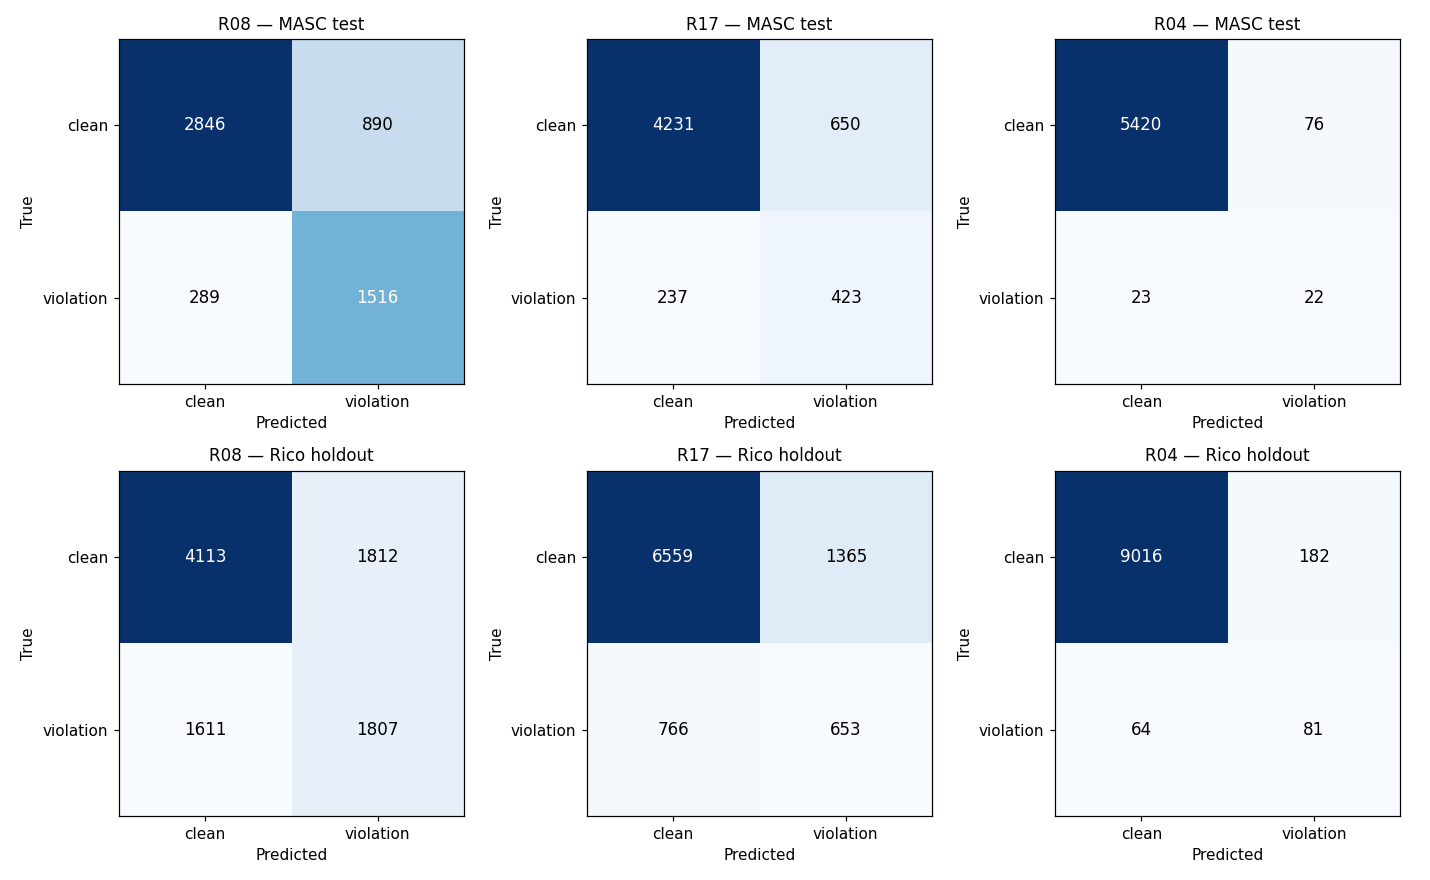
\includegraphics[width=0.85\textwidth]{swin_tiny_confusion_matrices.png}
\caption{Per-rule confusion matrices (R04, R17, R08) for the Swin-Tiny crop classifier on the MASC test split.}
\label{fig:swin_cm}
\end{figure*}

\begin{figure*}[!t]
\centering
\begin{subfigure}[t]{0.48\textwidth}
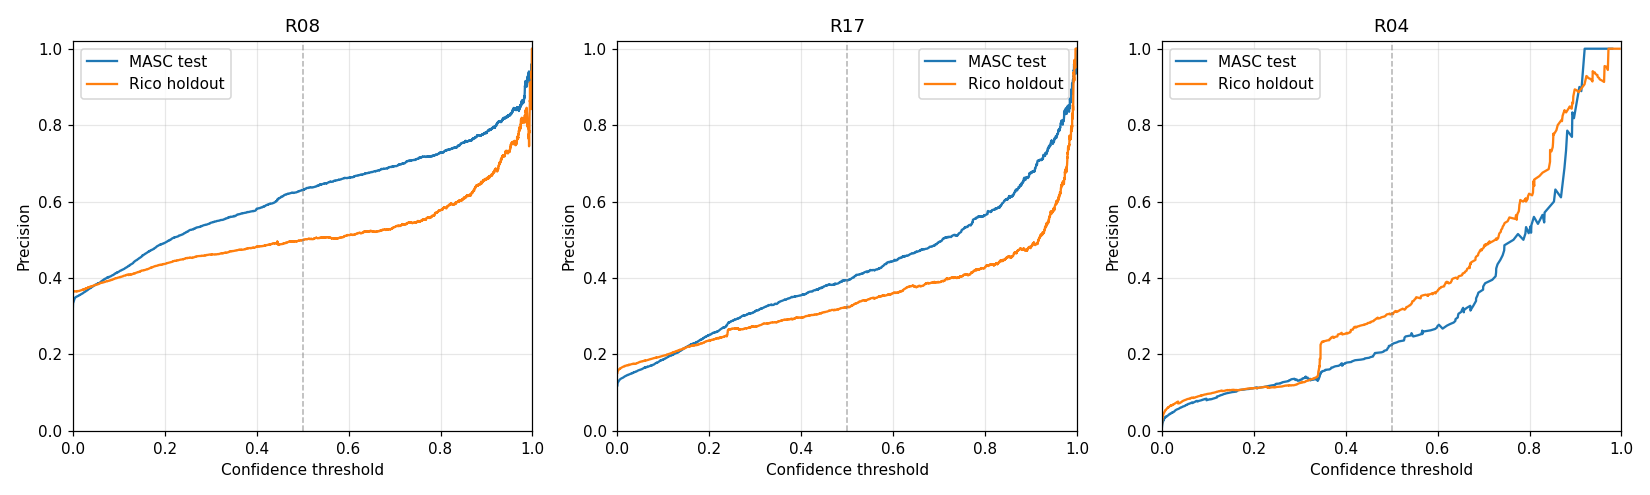
\includegraphics[width=\linewidth]{swin_tiny_p_curve.png}
\caption{Precision vs.\ threshold}
\end{subfigure}\hfill
\begin{subfigure}[t]{0.48\textwidth}
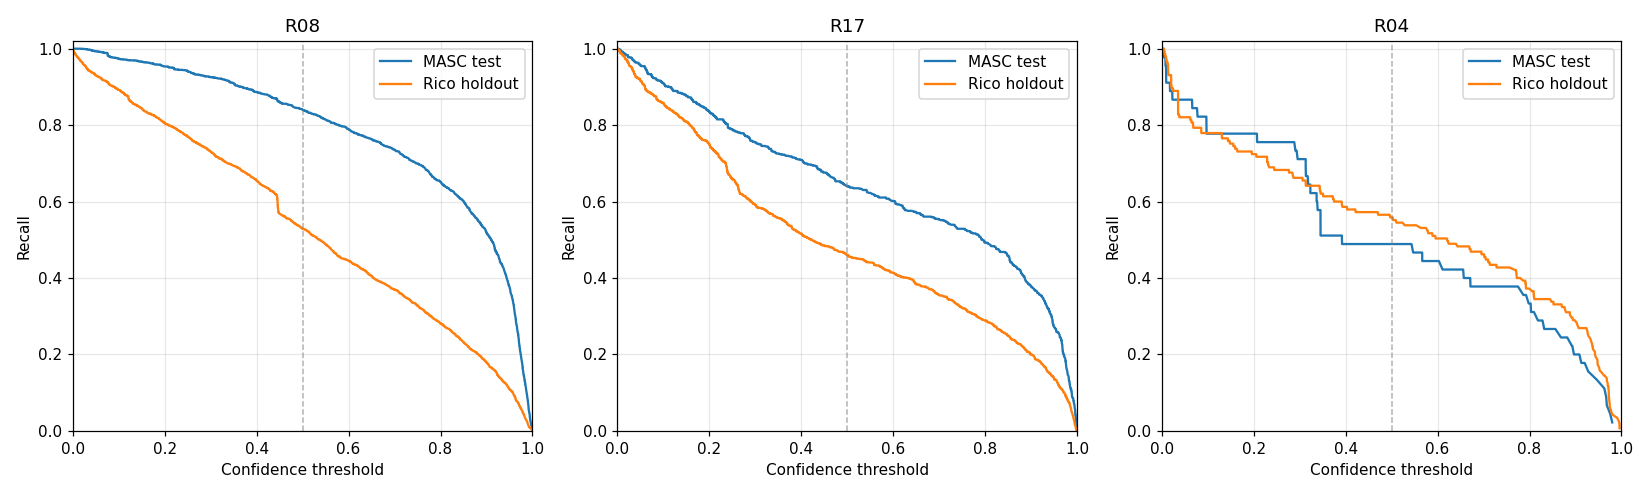
\includegraphics[width=\linewidth]{swin_tiny_r_curve.png}
\caption{Recall vs.\ threshold}
\end{subfigure}
\par\smallskip
\begin{subfigure}[t]{0.48\textwidth}
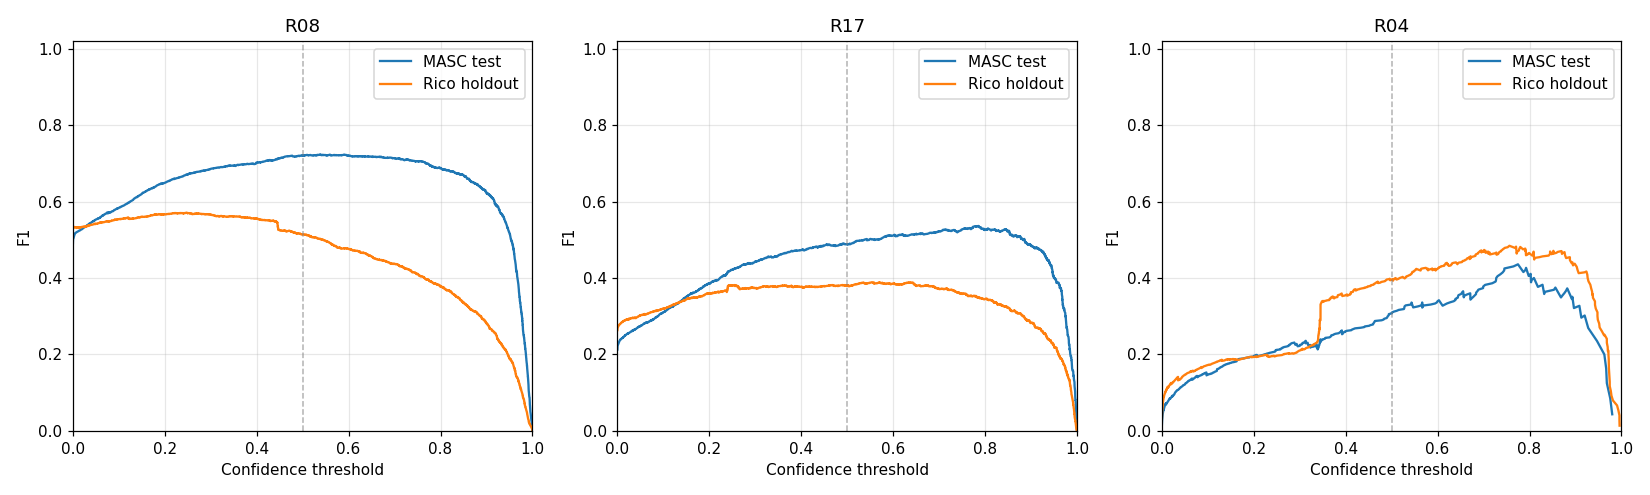
\includegraphics[width=\linewidth]{swin_tiny_f1_curve.png}
\caption{F1 vs.\ threshold}
\end{subfigure}\hfill
\begin{subfigure}[t]{0.48\textwidth}
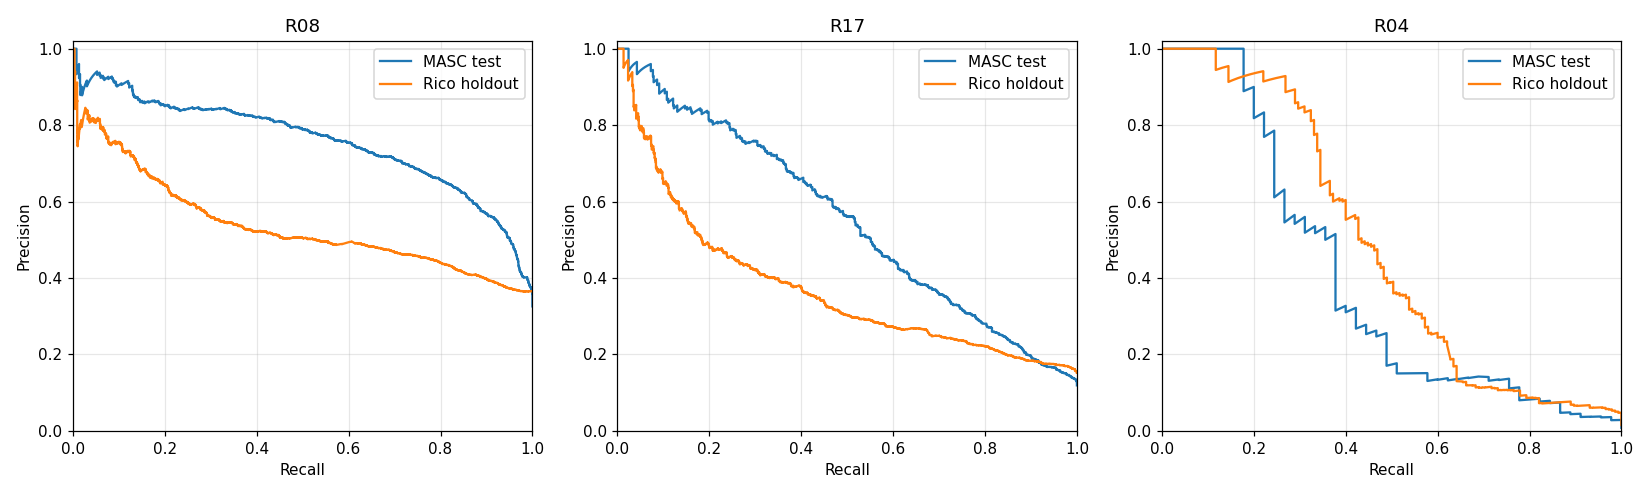
\includegraphics[width=\linewidth]{swin_tiny_pr_curves.png}
\caption{Precision--Recall (per rule)}
\end{subfigure}
\caption{Swin-Tiny crop classifier per-rule Precision, Recall, F1, and Precision--Recall curves, generated by \texttt{scripts/plot\_crop\_classifier\_curves.py} in the style of Ultralytics' auto-generated YOLO plots.}
\label{fig:swin_curves}
\end{figure*}

Figure~\ref{fig:swin_training} shows the resulting training curves; the frozen-backbone phase plateaus at val macro-F1 $\approx$0.20 before the backbone unfreeze produces a clear +37\% relative jump to a best of 0.274 at epoch 8, after which the model oscillates and early stopping triggers at epoch 13 (only the best-val-F1 checkpoint is ever kept). Figure~\ref{fig:swin_cm} and Figure~\ref{fig:swin_curves} give the per-rule confusion matrices and threshold-sweep curves for R04/R17/R08, the three rules with real positive training signal. Table~\ref{tab:swin} reports the final classification results on both the MASC test split and the Rico holdout.

\begin{table}[!t]
\caption{Crop-violation classifier (Swin-Tiny) results by rule.}
\label{tab:swin}
\centering
\scriptsize
\begin{tabular}{@{}lrrrr@{}}
\toprule
\textbf{Rule} & \textbf{MASC test F1} & \textbf{Support} & \textbf{Rico F1} & \textbf{Support} \\
\midrule
R04 & 0.31 & 45 & 0.40 & 145 \\
R17 & 0.49 & 660 & 0.38 & 1{,}419 \\
R08 & 0.72 & 1{,}805 & 0.51 & 3{,}418 \\
R09/R10/R28 & --- & 0 & --- & 0 \\
\midrule
\textbf{Macro avg.} & \textbf{0.25} & 2{,}510 & \textbf{0.22} & 4{,}982 \\
\bottomrule
\end{tabular}
\end{table}

R08, the rule with by far the most positive training examples, is the strongest signal (F1 0.72 on MASC test, 0.51 on Rico); R17 is usable (0.49/0.38); R04 is data-starved but still generalizes reasonably (0.31/0.40); R09, R10, and R28 report zero support because neither MASC nor Rico ever declares the raw color or text-size attributes those rules depend on -- a data-coverage gap in the source corpora, not a modeling failure. Rico macro-F1 (0.22) was the best result across the entire 33-backbone sweep and showed the tightest MASC-to-Rico generalization gap among top performers, consistent with the sweep's broader finding that attention-based backbones generalize measurably better than pure-CNN candidates on unseen apps. The classifier is wired into \texttt{backend/routers/audit.py}: \texttt{confirm\_violations()} runs immediately after rule checking and attaches an optional \texttt{cv\_confidence} score (0--1) to eligible R08/R17/R04 violations without ever overriding or removing a rule-detected violation. Figure~\ref{fig:cv-badge} shows how this confidence value surfaces in the Axion UI.

\begin{figure}[!t]
\centering
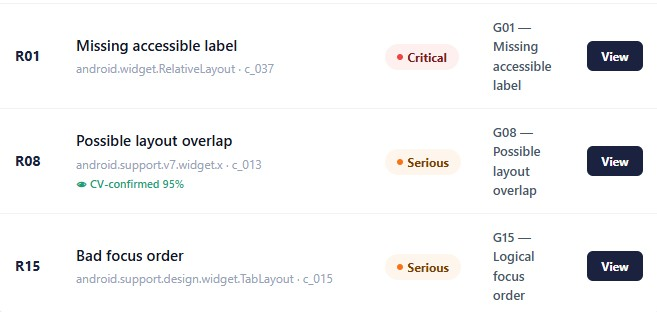
\includegraphics[width=\linewidth]{figma-11-cv-confidence-badge.jpg}
\caption{Axion issue detail view showing a rule-detected violation annotated with a computer-vision confidence badge.}
\label{fig:cv-badge}
\end{figure}

\subsection{Agentic Explanation Layer}
\texttt{src/agent.py} and \texttt{src/explainer.py} implement the LLM-driven enrichment stage. For every violation already present in \texttt{violations.json}, the agent generates three fields: a one-to-two sentence plain-English \texttt{agent\_explanation}, an \texttt{agent\_why\_it\_matters} statement describing impact on users with disabilities, and a concrete one-to-three line \texttt{agent\_developer\_fix} (e.g., an XML attribute change). Listing~\ref{lst:prompt} shows the structure of the per-violation prompt template.

\begin{lstlisting}[style=jsonstyle, caption={Per-violation agent prompt template.}, label={lst:prompt}]
System: Explain accessibility violations only.
        Never invent new violations.

User:
  rule_id: {rule_id}
  issue: {issue}
  component: {class, bounds, resource_id}
  guideline: {guideline}
  recommendation: {recommendation}

Return JSON: {agent_explanation,
              agent_why_it_matters,
              agent_developer_fix}
\end{lstlisting}

The system prompt explicitly instructs the model never to fabricate violations beyond those supplied, and the enrichment step is batched with an anti-hallucination match step that verifies returned explanations correspond to real input violation IDs. \texttt{src/llm\_providers.py} abstracts over four providers (Anthropic, OpenAI, Gemini, Groq) behind a common interface selected via the \texttt{LLM\_PROVIDER} environment variable; the deployed default is \textbf{Groq} (\texttt{llama-3.3-70b-versatile}), chosen after Anthropic and OpenAI were found to require paid billing and Gemini's free tier hit a quota bug during development. API timeouts or errors fall back to template-based explanations built directly from the rule engine's own \texttt{issue} and \texttt{recommendation} fields, so the pipeline never blocks on a network failure, and the LLM API key is used server-side only and never exposed to the browser.

\subsection{Report Generation}
\texttt{src/report.py} renders the enriched \texttt{report.json} into both an HTML report (Jinja2 template, with PIL-drawn bounding-box annotations on the screenshot) and a PDF export (the same HTML rendered to PDF via headless Chromium through Playwright), exposed via \texttt{GET} \url{/api/v1/audit/{id}/report/download?format=html|pdf}. Both formats include a cover section (screen ID, audit date, accessibility score, total violation count), a severity-ordered issue list (Critical/High first), and, per violation, the rule ID, WCAG reference, severity, affected component, agent explanation, impact statement, and developer fix. The 0--100 accessibility score is computed as

\begin{equation}
\begin{aligned}
\text{score} = \text{clamp}\big(100 - (20 \cdot n_{\text{crit}} + 10 \cdot n_{\text{high}} \\
{} + 5 \cdot n_{\text{med}} + 2 \cdot n_{\text{low}}),\ 0,\ 100\big)
\end{aligned}
\label{eq:score}
\end{equation}

and drives the Dashboard's circular score gauge. Figures~\ref{fig:dashboard} and \ref{fig:report-modal} show the resulting Dashboard, Issue Detail drawer, Audit Report page, and the Generate Report modal with its PDF layout.

\begin{figure}[!t]
\centering
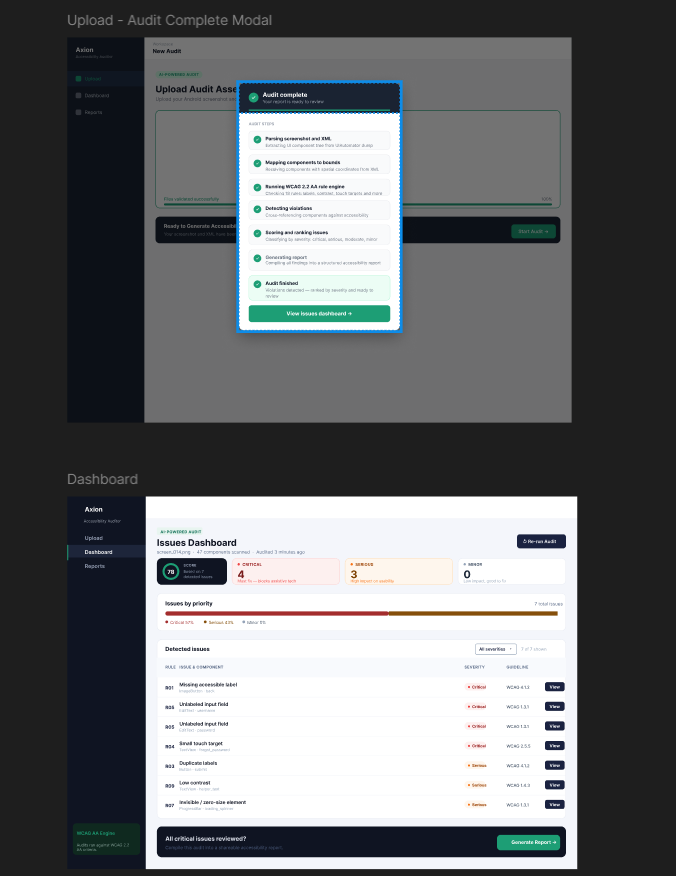
\includegraphics[width=\linewidth]{figma-05-audit-complete-dashboard.png}
\caption{Audit Complete modal (pipeline step checklist) and the Issues Dashboard: score gauge, severity summary cards, issues-by-priority bar, and violations table.}
\label{fig:dashboard}
\end{figure}

\begin{figure}[!t]
\centering
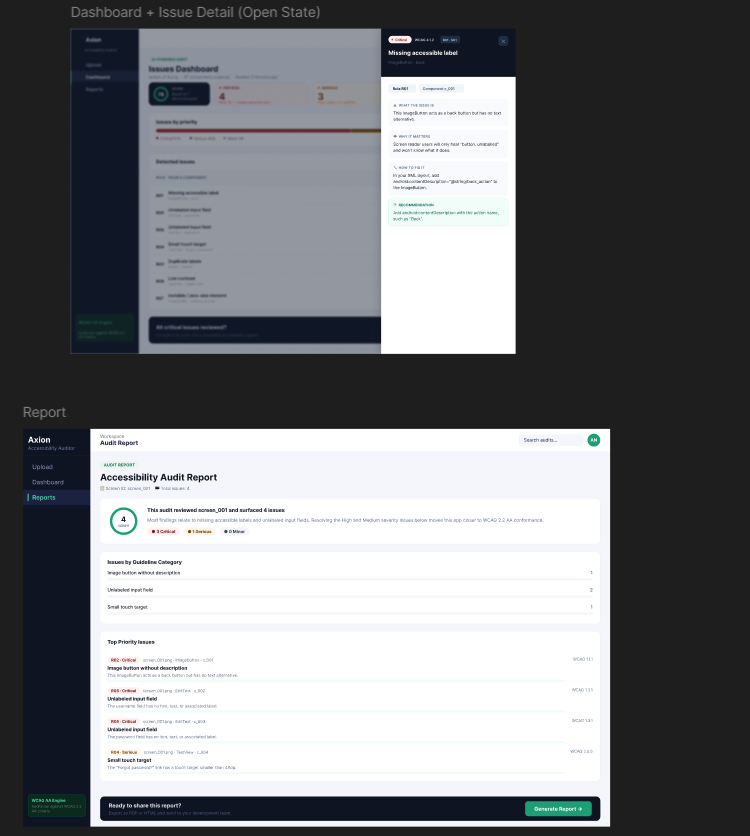
\includegraphics[width=\linewidth]{figma-06-dashboard-detail-report.png}
\caption{Issue Detail drawer (what the issue is / why it matters / how to fix it) and the Audit Report page with guideline-category breakdown.}
\label{fig:issue-detail}
\end{figure}

\begin{figure}[!t]
\centering
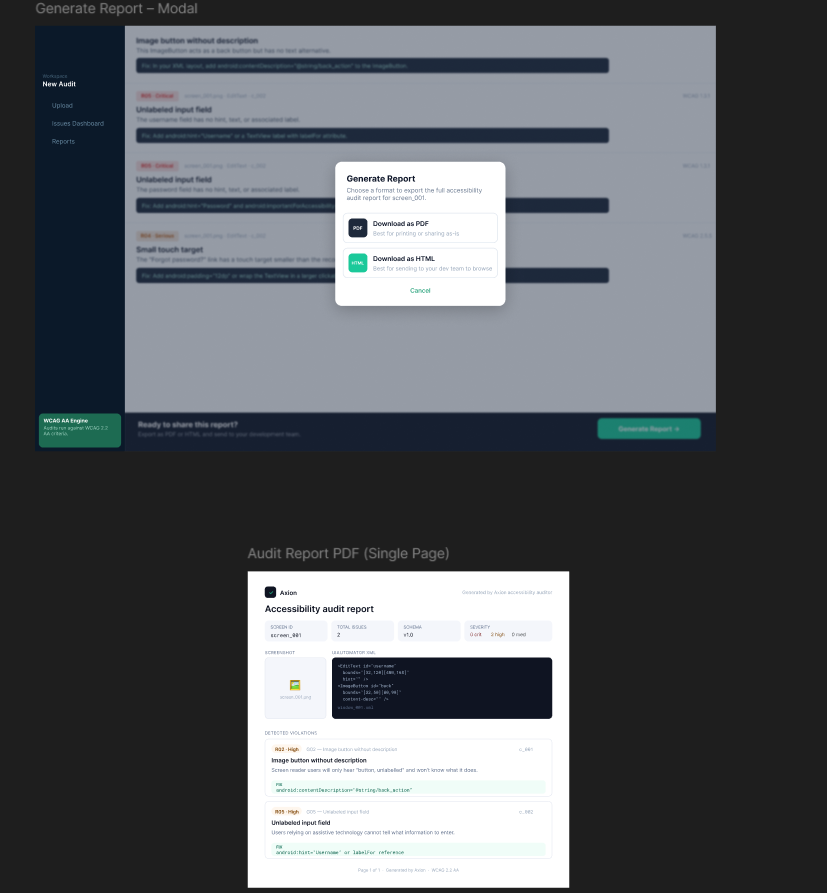
\includegraphics[width=\linewidth]{figma-07-generate-report-modal-pdf.png}
\caption{Generate Report modal (PDF/HTML download options) and the resulting exported PDF layout.}
\label{fig:report-modal}
\end{figure}

\subsection{Frontend: Axion}
The React 19 + Vite + Tailwind CSS frontend, designed first in Figma and implemented to match, provides Sign Up / Log In / Forgot Password flows (Figures~\ref{fig:signup} and \ref{fig:otp}), a sequential Upload flow, an Issues Dashboard with a slide-in Issue Detail drawer, an Audit Report screen with a Generate Report modal, and a Records page listing every past audit for the logged-in user with score, date, and severity summary. All authenticated screens share a persistent sidebar (logo, navigation, WCAG AA Engine badge) and a consistent dark-navy/teal (\texttt{\#0b1929}/\texttt{\#1bc99a}) visual identity, with primary action buttons kept always visible rather than hover-dependent -- a deliberate accessibility choice in the auditor's own interface.

\begin{figure*}[!t]
\centering
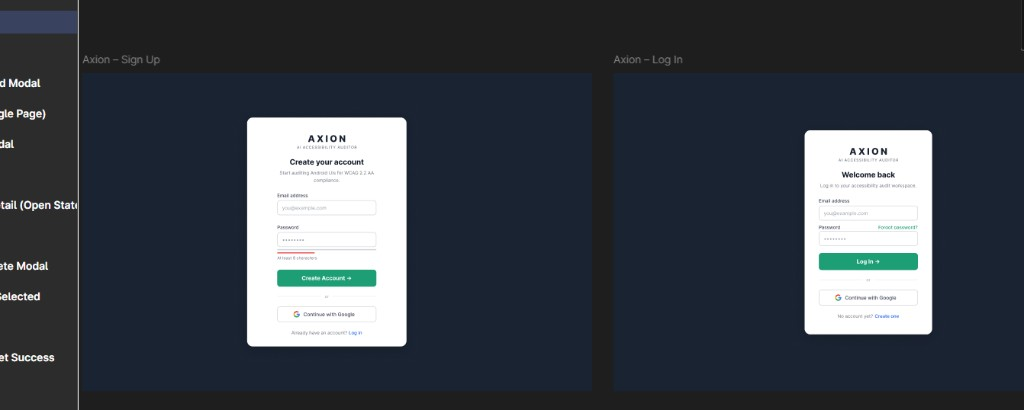
\includegraphics[width=0.75\textwidth]{figma-01-signup-login.png}
\caption{Axion Sign Up and Log In screens, with password strength hints and Google Sign-In.}
\label{fig:signup}
\end{figure*}

\begin{figure*}[!t]
\centering
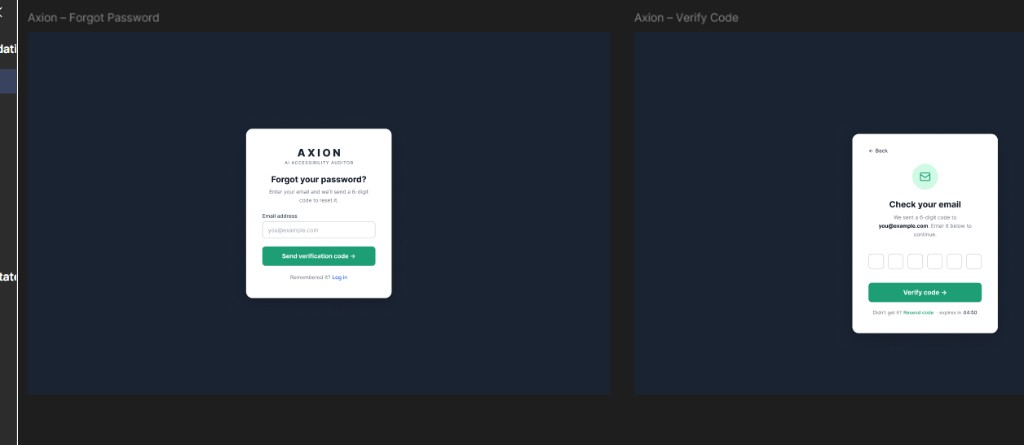
\includegraphics[width=0.85\textwidth]{figma-02-forgot-verify-otp.png}
\caption{Forgot Password flow: email entry and six-digit OTP verification with a resend countdown.}
\label{fig:otp}
\end{figure*}

\begin{figure}[!t]
\centering
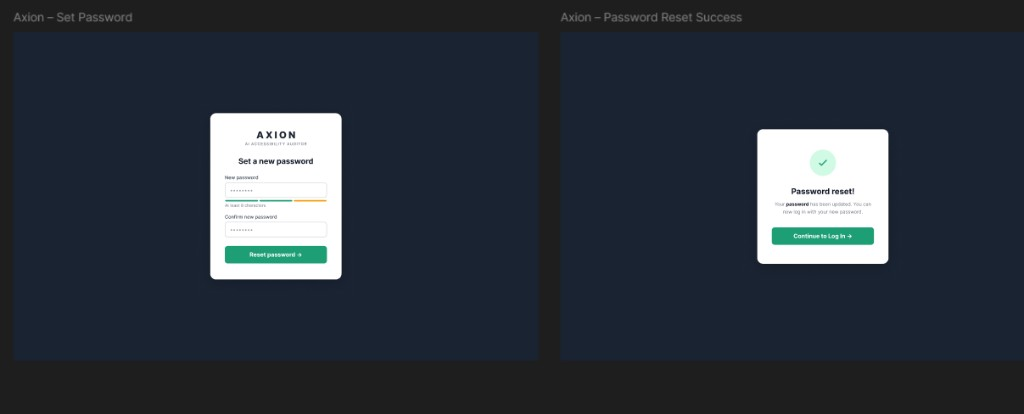
\includegraphics[width=\linewidth]{figma-03-reset-password-success.png}
\caption{Set Password screen and password-reset success confirmation.}
\label{fig:reset}
\end{figure}

\subsection{Authentication and Records}
User accounts are backed by JWT sessions, with registration and login accepting any valid email domain, a forgot-password flow that emails a six-digit, time-limited OTP via SMTP with resend support, and Google Sign-In via server-side ID-token verification against a configured \texttt{GOOGLE\_CLIENT\_ID}. Every completed audit is persisted against the authenticated \texttt{user\_id} in a flat JSON store (\texttt{backend/data/records.db.json}) recording screen ID, timestamp, violation counts by severity, accessibility score, original filenames, and artifact paths, exposed through user-scoped \texttt{GET}/\texttt{POST}/\texttt{DELETE} \texttt{/records} endpoints that never leak another user's records. This behavior was not always correct in practice: the frontend call that persists a completed audit had been documented as implemented since the design specification's first version but was never actually wired up, so audits completed and displayed correctly while silently never appearing in the user's history -- caught only by comparing the design documentation against the running frontend rather than by inspecting either in isolation, and fixed by adding the missing call with a duplicate-record guard. Table~\ref{tab:security} summarizes the security threats considered and their mitigations.

\begin{table}[!t]
\caption{Security threats and mitigations.}
\label{tab:security}
\centering
\scriptsize
\begin{tabular}{@{}p{2.3cm}p{5.3cm}@{}}
\toprule
\textbf{Threat} & \textbf{Mitigation} \\
\midrule
API key exposure & LLM calls made server-side only \\
JWT theft & HTTPS in production; httpOnly cookie option (Stretch) \\
XXE injection & Safe XML parsing, no external entity resolution \\
Upload abuse & 20 MB per-file limit, MIME validation \\
Path traversal & Sanitized paths in Records service \\
Cross-user access & JWT \texttt{user\_id} scoping on every records query \\
OTP brute force & Rate limiting and expiry countdown \\
\bottomrule
\end{tabular}
\end{table}

\subsection{Deployment}
The system ships as a three-service Docker Compose topology -- \texttt{backend} (FastAPI + pipeline, port 8000 internally), \texttt{auditor} (a batch worker running the parser/rule pipeline over a mounted dataset), and \texttt{frontend} (Vite dev server, port 5173) -- on an internal bridge network, started with a single documented command (\texttt{docker compose up --build}). Two real deployment bugs were found and fixed by actually building and running the containers rather than assuming the compose file was correct: the backend's \texttt{requirements.txt} was missing the \texttt{torch}/\texttt{torchvision}/\texttt{timm}/\texttt{ultralytics} dependencies pulled in by the two CV modules, causing a startup crash, and after that fix the container still failed with \texttt{ImportError: libxcb.so.1} because \texttt{ultralytics} depends on the full GUI-capable \texttt{opencv-python} rather than the headless variant, requiring several system libraries (\texttt{libgl1}, \texttt{libglib2.0-0}, \texttt{libsm6}, \texttt{libxext6}, \texttt{libxrender1}) not present in the base \texttt{python:3.11-slim} image.

A further, structurally similar bug surfaced only when deploying to a second, GPU-equipped machine: the backend image's build context had been the \texttt{backend/} subdirectory, so it never actually packaged the repository-root \texttt{src/} and \texttt{models/} directories that the pipeline imports at runtime, working locally only because development compose bind-mounts the whole repository over the container at runtime. A standalone container built from that image and run without the bind mount -- exactly the deployment scenario on the second machine -- failed immediately with a missing-module error. The fix changes the build context to the repository root and copies \texttt{src/}, \texttt{models/}, and \texttt{backend/} explicitly, making the image genuinely self-contained. The \texttt{backend} service also gained an NVIDIA GPU reservation (Docker Compose's \texttt{deploy.resources.reservations.devices}), and its externally published port was made configurable (\texttt{8001} rather than \texttt{8000}, with the container's internal port unchanged) to accommodate the target lab machine's port 8000 already being in use by unrelated services -- both changes verified by a full audit, including the screenshot-only detection path, completing successfully end to end on that machine with GPU acceleration active.

\subsection{Testing}
The complete pytest suite comprises 155 tests spanning the parser (including MASC wrapper-nesting edge cases), the R01--R30 rule engine against 61 controlled pass/fail XML fixtures, the agent's score formula and template fallback, the report generator's HTML/PDF export, the FastAPI audit routes (including CV-wiring and YOLO-fallback behavior), and a dedicated 22-test authentication suite (JWT, OTP, Google OAuth, records isolation). Integration-level sign-off scripts additionally re-run the full pipeline against the entire MASC corpus and the Rico holdout after every significant rule or parser change, giving dataset-scale regression coverage beyond the unit fixtures.

\section{Evaluation Methodology}

Evaluation combined several complementary methods, aligned with the project's QA test plan: (1) 10--15 controlled XML fixtures with known expected violations, used as unit-level regression tests for R01--R05 and beyond; (2) full-pipeline runs across 25--40 curated screens with manual labeling of each detected violation as Correct / False Positive / Missed (Week 6, 40 stratified-random screens -- four per MASC category, seed \texttt{20260715} for reproducibility); (3) rule-wise and guideline-wise aggregate QA summaries across a larger MASC sample and the full Rico holdout (Week 7); and (4) a final batch evaluation of the entire 1{,}698-screen Rico holdout with zero pipeline failures, giving both a health snapshot of the rule engine at scale and a genuine unseen-data generalization check for the two CV models.

\section{Results}

\subsection{Manual Review (Week 6, 40 Screens)}
Across the 40 stratified-random MASC screens manually reviewed, 35 of 40 were classified \texttt{mostly\_agree} or \texttt{agree\_clean} between the rule engine's findings and human judgment, with the remaining 5 flagged \texttt{over\_flagging} or \texttt{mixed\_r30\_noise}. Three recurring false-positive themes were identified -- R07/R08 nesting of a parent clickable container against children whose text already names the control, borderline contrast flags on secondary chrome elements by design, and R30 density from scroll-list icon repeats -- all three of which motivated the Week 8 rule-accuracy fixes described above. Recurring miss themes (issues real but outside the static XML's reach) included live/dynamic announcements such as chat unread badges, field--error association on auth forms, and selected-state on bottom navigation tabs when the XML lacks state attributes.

\subsection{Rule Engine at Scale (Rico Holdout)}
Table~\ref{tab:ricoagg} summarizes the aggregate health of the rule engine over the full 1{,}698-screen Rico holdout, run after the Week 8 accuracy fixes.

\begin{table}[!t]
\caption{Rico holdout aggregate rule-engine results (1,698/1,698 screens, 0 failures).}
\label{tab:ricoagg}
\centering
\scriptsize
\begin{tabular}{@{}lr@{}}
\toprule
\textbf{Metric} & \textbf{Value} \\
\midrule
Mean violations / screen & 31.7 \\
Median violations / screen & 14 \\
Mean accessibility score (0--100) & 32.0 \\
Screens with zero violations & 87 \\
\bottomrule
\end{tabular}
\end{table}

Table~\ref{tab:topguidelines} lists the most frequently triggered guidelines across the holdout by screen coverage. Missing/absent accessible labels (G01/G02/G30) and zero-area or invalid-bounds elements (G07/G25, which share detection logic) dominate, appearing on 63--85\% of screens; several guidelines that depend on declared color or text-size attributes (G09, G10, G22, G28, G29) never fire on either corpus, a data-coverage limitation of the source XML rather than a rule defect.

\begin{table}[!t]
\caption{Top guidelines by screen coverage, Rico holdout (1,698 screens).}
\label{tab:topguidelines}
\centering
\scriptsize
\begin{tabular}{@{}p{1.5cm}p{3.4cm}r@{}}
\toprule
\textbf{ID} & \textbf{Guideline (short)} & \textbf{\% screens} \\
\midrule
G01/G02/G30 & Missing / absent accessible labels & 85.3\% \\
G07/G25 & Zero-area or unpausable/invalid elements & 63.5\% \\
G18 & Multi-finger-only interaction & 47.0\% \\
G16 & Decorative element left in focus tree & 49.5\% \\
G15 & Focus order not top-to-bottom & 46.4\% \\
G08 & Overlapping content/focus order & 27.5\% \\
G17 & Insufficient touch-target spacing & 28.4\% \\
\bottomrule
\end{tabular}
\end{table}

The most frequently triggered individual rules were R07 (zero/invalid-bounds elements, 63.5\% of screens), R01 (missing accessible label, 85.3\% of screens), and R08 (layout overlap, 27.5\% of screens); R09, R10, R20, R22, R25, R28, and R29 never fired on the holdout, consistent with the underlying data-coverage gap rather than a rule-logic failure. Manual QA classified the dominant residual noise pattern as clickable-container-vs-child overlap and repeated icon instances -- exactly the two patterns the Week 8 R08/R30 fixes targeted, confirmed by the -43.2\% R08 reduction reported in Section~V-C.

\subsection{Computer-Vision Modules}
Both stretch computer-vision modules were trained to completion, evaluated on the unseen Rico holdout, and wired into the production backend pipeline rather than left as standalone notebooks. The YOLO detector (Table~\ref{tab:yolo}, Figures~\ref{fig:yolo_results}--\ref{fig:yolo_cm}) demonstrated a genuine, if moderate, generalization signal -- roughly a $10\times$ mAP50 lift over its untrained base on unseen apps. The Swin-Tiny crop classifier (Table~\ref{tab:swin}, Figures~\ref{fig:swin_training}--\ref{fig:swin_curves}) achieved its best Rico holdout macro-F1 (0.22) of any of the 33 backbones evaluated in the comparison sweep, with the tightest MASC-to-Rico generalization gap among the top performers.

\subsection{System-Level Validation}
The complete pytest suite (155 tests) passed in full. All 99 functional and non-functional requirements tracked in the project's requirements traceability matrix were marked Done by project close, including both Stretch computer-vision integrations, which were initially deferred and completed only in the final week of the internship.

\section{Discussion and Limitations}

Several limitations are worth stating explicitly rather than glossing over. First, the primary rule-detection accuracy is bounded by what the source datasets actually declare: MASC and Rico XML dumps never populate the raw color or text-size attributes that R09 (contrast), R28 (font-scale overflow), and R29 (all-caps body text) depend on, so those rules are correctly implemented but structurally inactive on the available corpora -- a data-coverage gap rather than a code defect. Second, both computer-vision modules, while genuinely wired into the pipeline and showing real (not memorized) generalization to the unseen Rico holdout, report modest absolute accuracy (macro-F1 0.22, mAP50 0.25); they are positioned as supplementary confidence signals that never override the deterministic rule engine, not as a replacement for it. Third, the crop classifier could only be trained with real positive examples for R08, R17, and R04 -- R09/R10/R28 have zero positive training crops for the same data-coverage reason described above, so \texttt{confirm\_violations()} deliberately restricts itself to the three rules with genuine signal. Finally, the prototype's persistence layer is a flat JSON store rather than a production database, and its authentication/authorization is JWT-based rather than enterprise SSO -- both explicit, documented scope decisions appropriate for an eight-week research prototype rather than a production system.

\section{Future Work}

Directions identified but not pursued within the internship's scope include: a dedicated pixel-sampling contrast module that measures rendered foreground/background colors directly from the screenshot rather than relying on declared XML attributes, closing the R09 data-coverage gap independently of dataset limitations; specialized detectors for visual text clipping to give R10/R28 a real signal; interactive click-to-highlight linking between the HTML report and the screenshot; a curated, manually validated benchmark dataset released as a project deliverable; and batch/CLI evaluation tooling suitable for continuous-integration regression testing of the rule engine against the full MASC and Rico corpora on every code change.

\section{Conclusion}

This internship delivered a complete, end-to-end Agentic Accessibility Auditor for Android UIs: a deterministic 30-rule engine mapped to 30 WCAG-aligned guidelines, an LLM-based explanation layer constrained to never fabricate findings, an HTML/PDF report generator, a fully authenticated React dashboard with per-user audit history, and -- beyond the original Must-Have scope -- two trained and backend-integrated computer-vision models providing a screenshot-only fallback detector and pixel-level rule confirmation. The system was developed against a 7{,}068-screen dataset and validated, without tuning, on a disjoint 1{,}698-screen holdout, with all 99 tracked requirements and 155 automated tests passing at project close. The result is a practical demonstration that combining a deterministic, auditable rule engine with a tightly scoped LLM explanation layer can produce accessibility tooling that is both more thorough than screenshot-only scanners and more explainable than a black-box classifier.

\section*{Acknowledgment}
The authors thank their team lead and the FAST--NUCES internship supervisors for guidance throughout the eight-week program, and acknowledge the creators of the MASC and Rico datasets, without which the parser, rule engine, and computer-vision modules described here could not have been developed or evaluated.

\begin{thebibliography}{9}

\bibitem{wcag} World Wide Web Consortium (W3C), ``Web Content Accessibility Guidelines (WCAG) 2.2,'' W3C Recommendation, 2023.

\bibitem{uiautomator} Android Developers, ``Write automated tests with UI Automator,'' Google, 2026. [Online]. Available: \url{https://developer.android.com/training/testing/other-components/ui-automator}

\bibitem{ieee830} IEEE, ``IEEE Std 830-1998: Recommended Practice for Software Requirements Specifications,'' Institute of Electrical and Electronics Engineers, 1998.

\bibitem{yolo} G. Jocher et al., ``Ultralytics YOLO11,'' Ultralytics, 2024.

\bibitem{swin} Z. Liu, Y. Lin, Y. Cao, H. Hu, Y. Wei, Z. Zhang, S. Lin, and B. Guo, ``Swin Transformer: Hierarchical Vision Transformer using Shifted Windows,'' in \emph{Proc. IEEE/CVF Int. Conf. Computer Vision (ICCV)}, 2021, pp. 10012--10022.

\bibitem{rico} B. Deka et al., ``Rico: A Mobile App Dataset for Building Data-Driven Design Applications,'' in \emph{Proc. 30th Annual ACM Symp. User Interface Software and Technology (UIST)}, 2017.

\bibitem{masc-kaggle} A. A. Ahmed, ``MASC Dataset,'' Kaggle, 2023. [Online]. Available: \url{https://doi.org/10.34740/kaggle/ds/3962521}

\bibitem{rico-kaggle} Kaggle user \texttt{onurgunes1993}, ``RICO Dataset,'' Kaggle. [Online]. Available: \url{https://www.kaggle.com/datasets/onurgunes1993/rico-dataset}

\bibitem{screenaudit} M. Zhong, R. Chen, X. Chen, J. Fogarty, and J. O. Wobbrock, ``ScreenAudit: Detecting Screen Reader Accessibility Errors in Mobile Apps Using Large Language Models,'' in \emph{Proc. ACM CHI Conf. Human Factors in Computing Systems (CHI)}, 2025.

\bibitem{insight} J. O. Ansah, A. Kapoor, A. Khanna, M. Vinod, P. Njeck, and S. Gao, ``Insight: Enhancing Mobile Accessibility for Blind and Visually Impaired Users with LLMs,'' arXiv:2605.09803, 2026.

\bibitem{fastapi} S. Ramirez, ``FastAPI Documentation,'' 2024. [Online]. Available: https://fastapi.tiangolo.com

\bibitem{react} Meta Platforms, ``React 19 Documentation,'' 2024.

\end{thebibliography}

\end{document}
